\section{Compressão para Microserviços}

\begin{frame}{Compressão de modelos para microserviços}
    \begin{itemize}
        \item Microserviços são um estilo arquitetural que tem ganhado crescente popularidade nos últimos anos devido à sua abordagem ágil e escalável para o desenvolvimento de aplicações;
        \item Em ambientes de microserviços, o uso de recursos é uma preocupação importante;
        \item Modelos de DNNs, especialmente os mais complexos, podem requisitar um grande consumo de memória, processamento e tempo de inferência. O que pode ser problemático para esses ambientes.
        \item O uso de estratégias de compressão de modelos de DNN pode afetar positivamente o desempenho e uso eficiente dos recursos computacionais de microserviços;
    \end{itemize}
\end{frame}


\begin{frame}{Compressão de modelos para microserviços}
    \begin{itemize}
        \item A compressão de modelos também pode tornar a implementação e a escalabilidade dos microserviços mais ágeis;
        \item Modelos menores são mais rápidos de transferir e carregar em diferentes ambientes, tornando o processo de implantação mais eficiente.
    \end{itemize}
\end{frame}

\begin{frame}{Dataset}
    \begin{figure}[H]
    \centering
    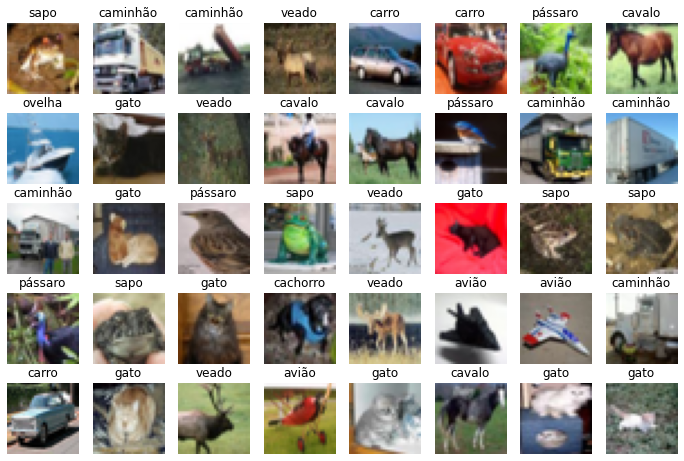
\includegraphics[width=0.65\textwidth]{figuras/cifar10ex.png}
    \caption{Amostra do dataset cifar10}
    \end{figure}
\end{frame}

\begin{frame}{Treinamento da DNN}
    Para o treinamento do modelo, foram escolhidos os seguintes parâmetros:
    \begin{itemize}
        \item Tamanho de cada lote de 64;
        \item Otimizador de Descida de Gradiente Estocástico (SGD);
        \item 60 mil amostras para treino e 10 mil para validação;
        \item Taxa de aprendizagem de 0,05 e momento do 0,9;
        \item Critétio de loss como entropia cruzada de categoria.
    \end{itemize}
\end{frame}

\begin{frame}{Arquitetura do modelo}
O modelo foi definido com a arquitetura VGG16 com duas camadas densas:
\begin{columns}[T,c]
    \column{.5\textwidth}
      \scriptsize
      \begin{itemize}
        \item Entrada($32 \times 32 \times 3$);
        \item Conv2D($64 \times 3 \times 3$) e ReLU;
        \item Conv2D($64 \times 3 \times 3$) e ReLU;
        \item MaxPool($2 \times 2$);
        \item Conv2D($128 \times 3 \times 3$) e ReLU;
        \item Conv2D($128 \times 3 \times 3$) e ReLU;
        \item MaxPool($2 \times 2$);
        \item Conv2D($256 \times 3 \times 3$) e ReLU;
        \item Conv2D($256 \times 3 \times 3$) e ReLU;
        \item Conv2D($256 \times 3 \times 3$) e ReLU;
        \item MaxPool($2 \times 2$);
      \end{itemize}
    \column{.5\textwidth}
      \scriptsize
      \begin{itemize}
        \item Conv2D($512 \times 3 \times 3$) e ReLU;
        \item Conv2D($512 \times 3 \times 3$) e ReLU;
        \item Conv2D($512 \times 3 \times 3$) e ReLU;
        \item MaxPool($2 \times 2$);
        \item Conv2D($512 \times 3 \times 3$) e ReLU;
        \item Conv2D($512 \times 3 \times 3$) e ReLU;
        \item Conv2D($512 \times 3 \times 3$) e ReLU;
        \item MaxPool($2 \times 2$);
        \item Dense($4096$) e ReLU;
        \item Dense($4096$) e ReLU;
        \item Dense($10$) e Softmax.
      \end{itemize}
    \end{columns}
\end{frame}

\begin{frame}{Resultados do treinamento}
    \scriptsize
    \begin{table}[H]
        \caption{\scriptsize{Acurácias obtidas na classificação de imagens a partir do modelo comprimido para vários valores de quantidade de bits e $\alpha$.}}
        \centering
        \begin{tabular}{l|llll}
        \hline
        \textbf{\diagbox{bits}{$\alpha$}} & \textbf{0,00}  & \textbf{0,50} & \textbf{1,50} & \textbf{1,25}\\ \hline
        \textbf{32 bits} &	81,58\%	& 79,39\% & 79,53\% & 74,64\%\\
        \textbf{8 bits} & 79,76\%	& 80,77\% & 79,31\% & 74,42\%\\\hline
        \end{tabular}
        \end{table}
    \scriptsize
    \begin{table}[H]
        \caption{\scriptsize{Esparsidades obtidas na classificação de imagens a partir do modelo comprimido para vários valores de tamanho de bits e $\alpha$.}}
        \centering
        \begin{tabular}{l|lll}
        \hline
        \textbf{\diagbox{bits}{$\alpha$}}  & \textbf{0,50} & \textbf{1,50} & \textbf{1,25}\\ \hline
        \textbf{32 bits} & 37,92\% & 62,76\% & 74,76\%\\
        \textbf{8 bits} & 36,94\% & 60,68\% & 74,49\%\\\hline
        \end{tabular}
        \end{table}
\end{frame}

\begin{frame}{Resultados do treinamento}
    \begin{figure}[H]
  \centering

  \begin{subfigure}[b]{0.49\textwidth}
    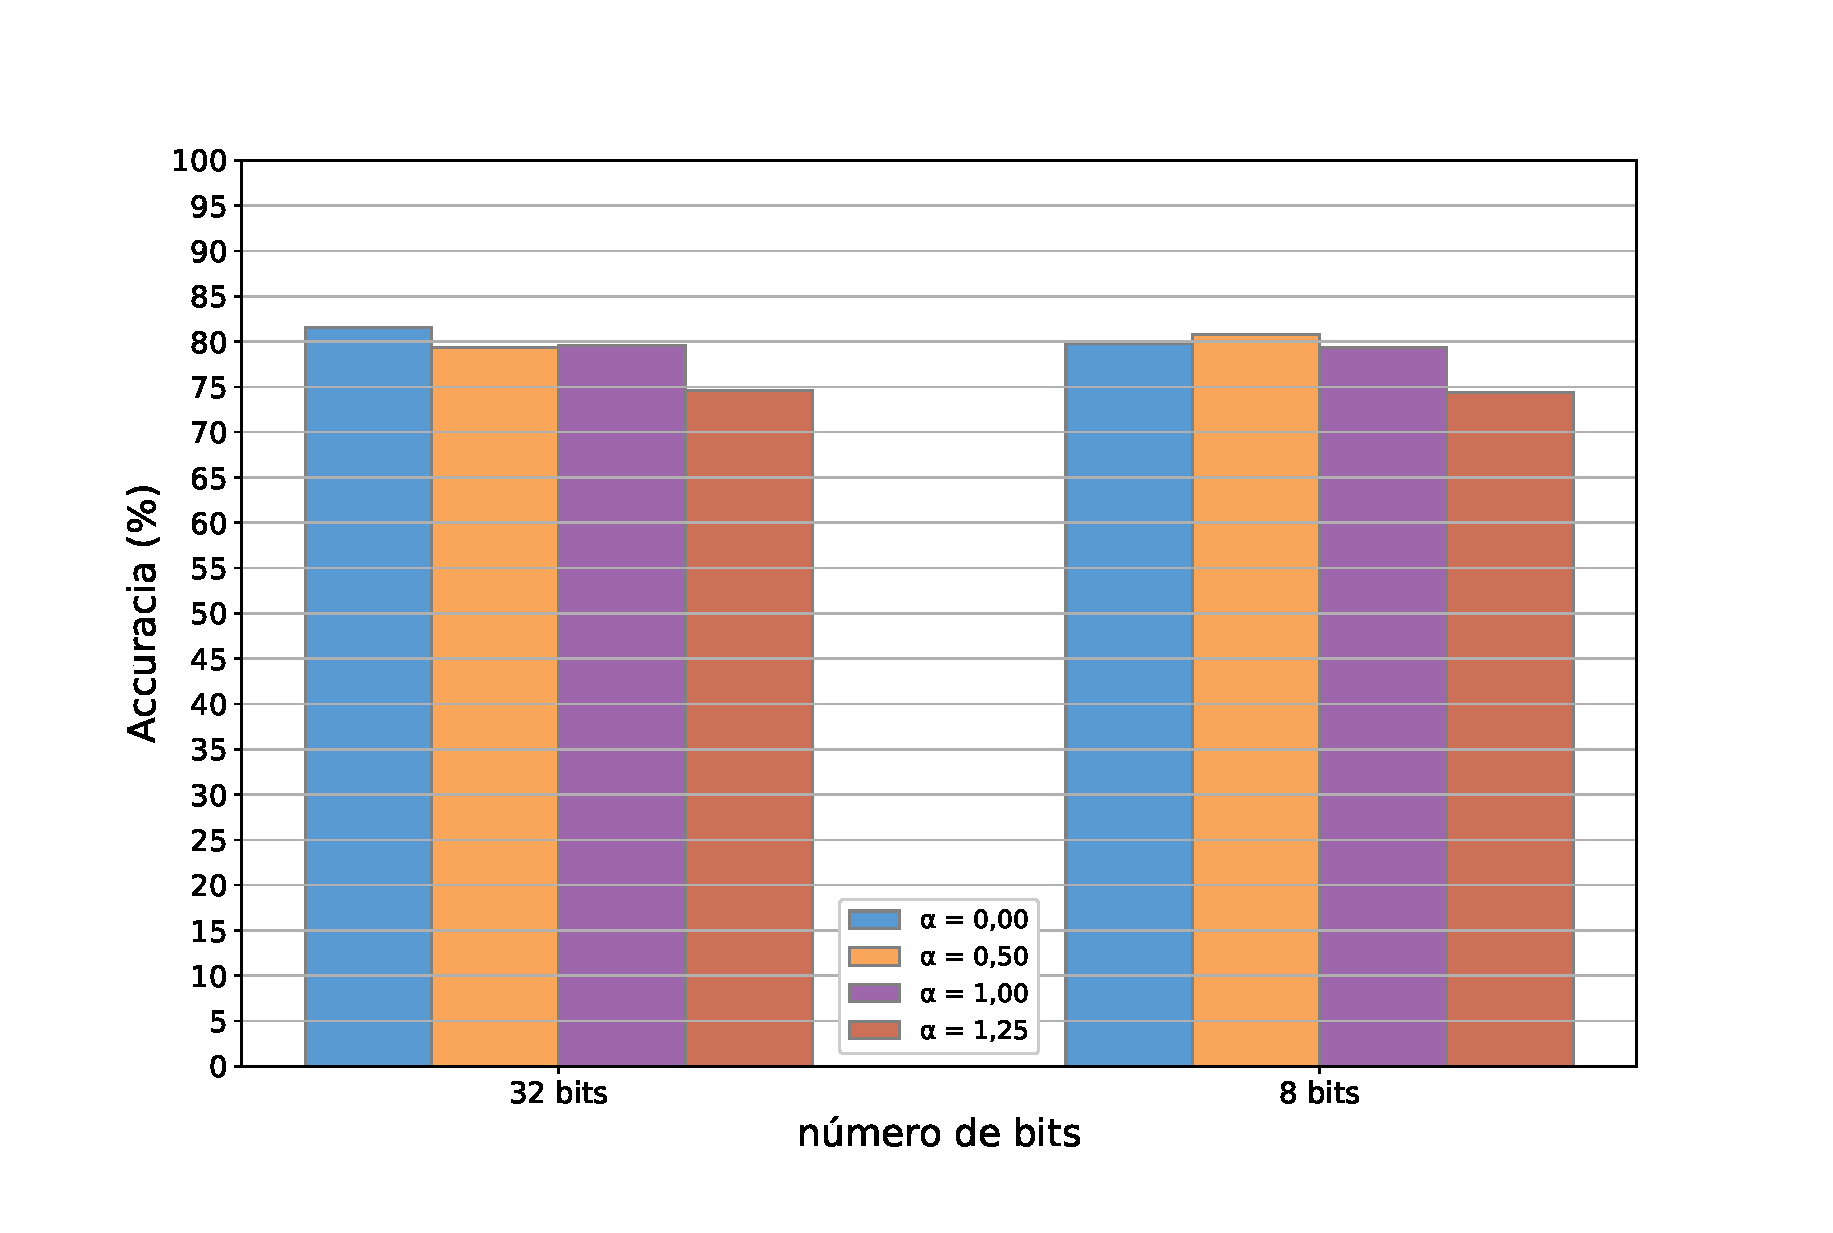
\includegraphics[width=\textwidth]{figuras/cifar_acc_fig.eps}
    \caption{Acurácia dos modelos}
  \end{subfigure}
  \hfill
  \begin{subfigure}[b]{0.49\textwidth}
    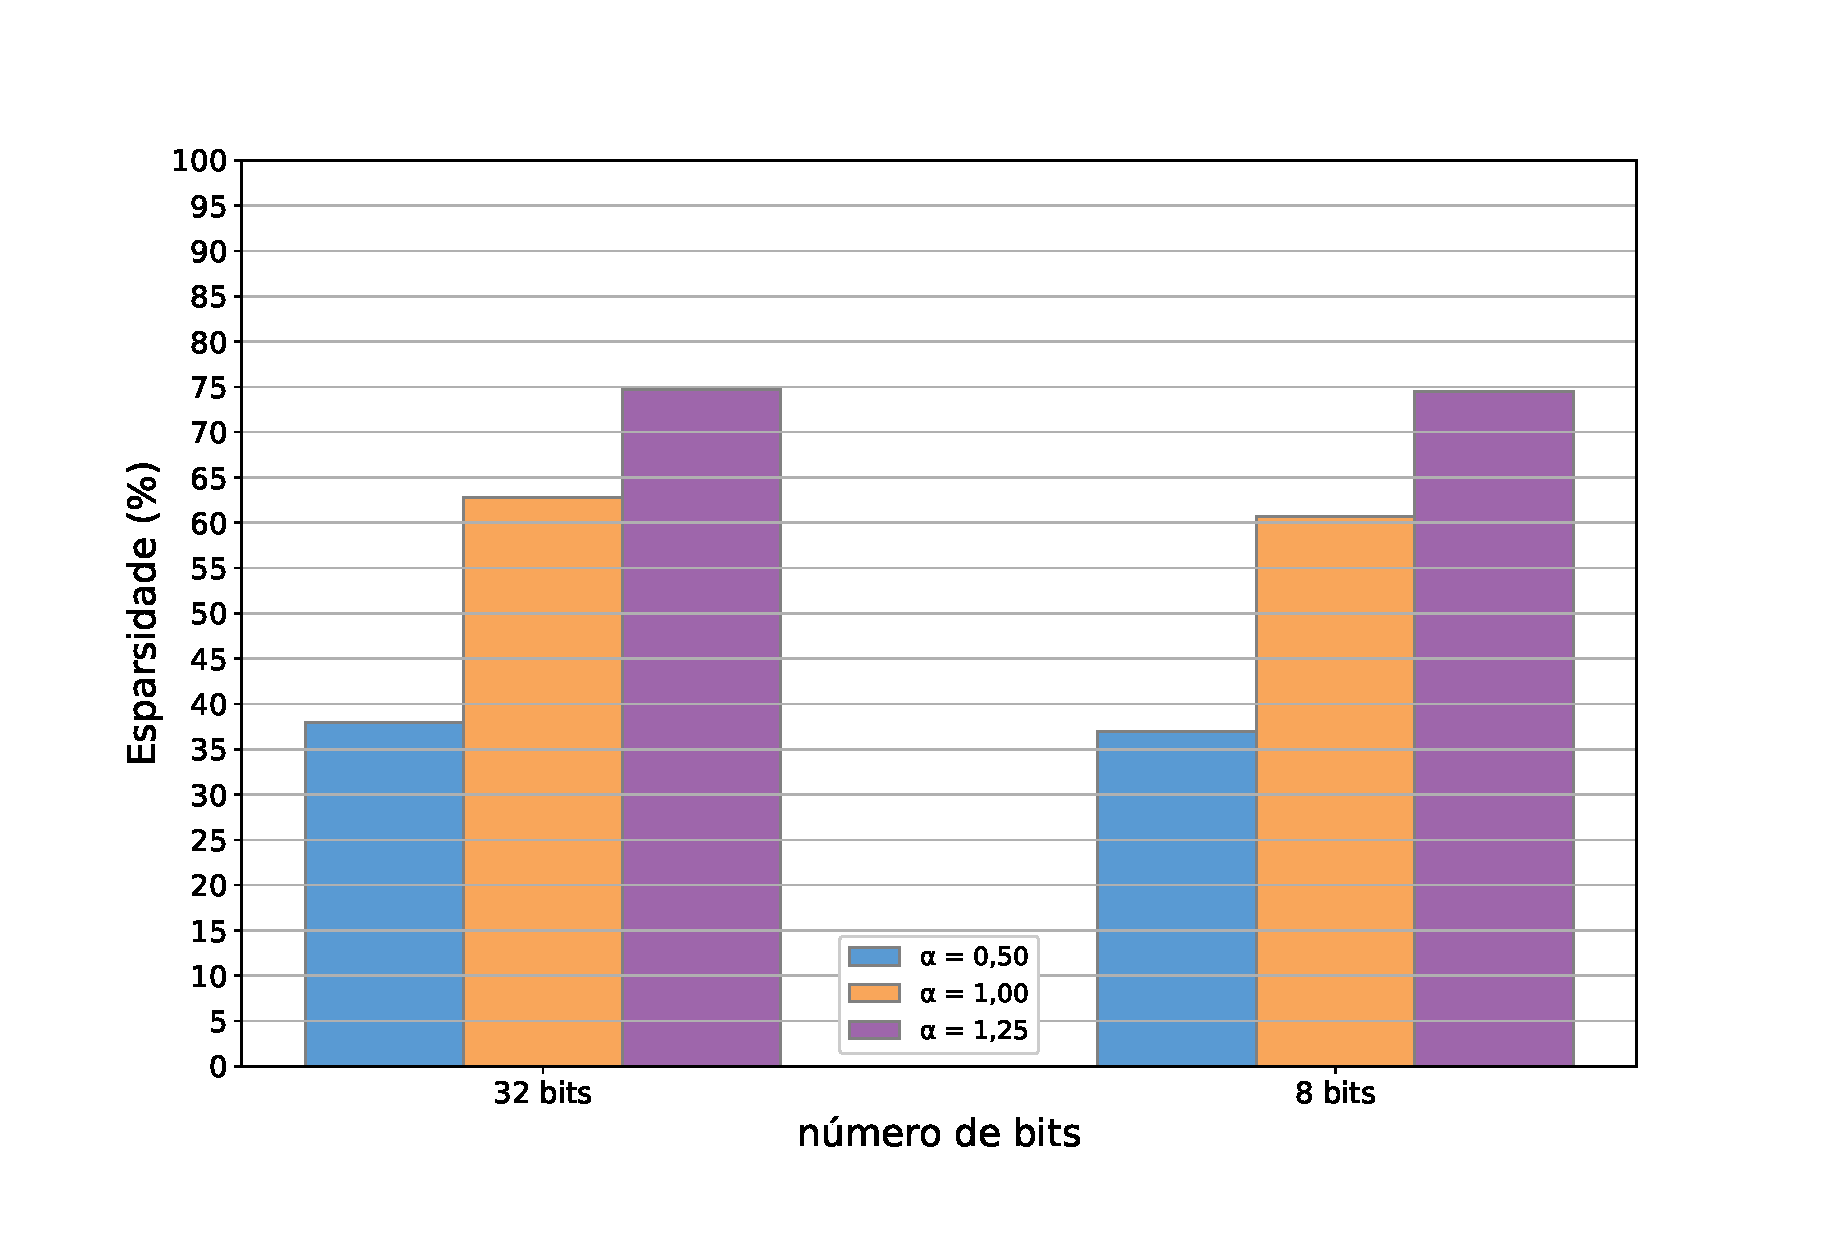
\includegraphics[width=\textwidth]{figuras/cifar_sparsity_fig.eps}
    \caption{Esparsidade dos modelos}
  \end{subfigure}
  \caption{Acurácias e esparsidades obtidas na classificação de imagens a partir do modelo comprimido para vários valores de tamanho de bits e $\alpha$.}
  \end{figure}
\end{frame}

\begin{frame}{Resultados do treinamento}
    \begin{figure}[H]
        \centering
        \begin{subfigure}[b]{0.49\textwidth}
          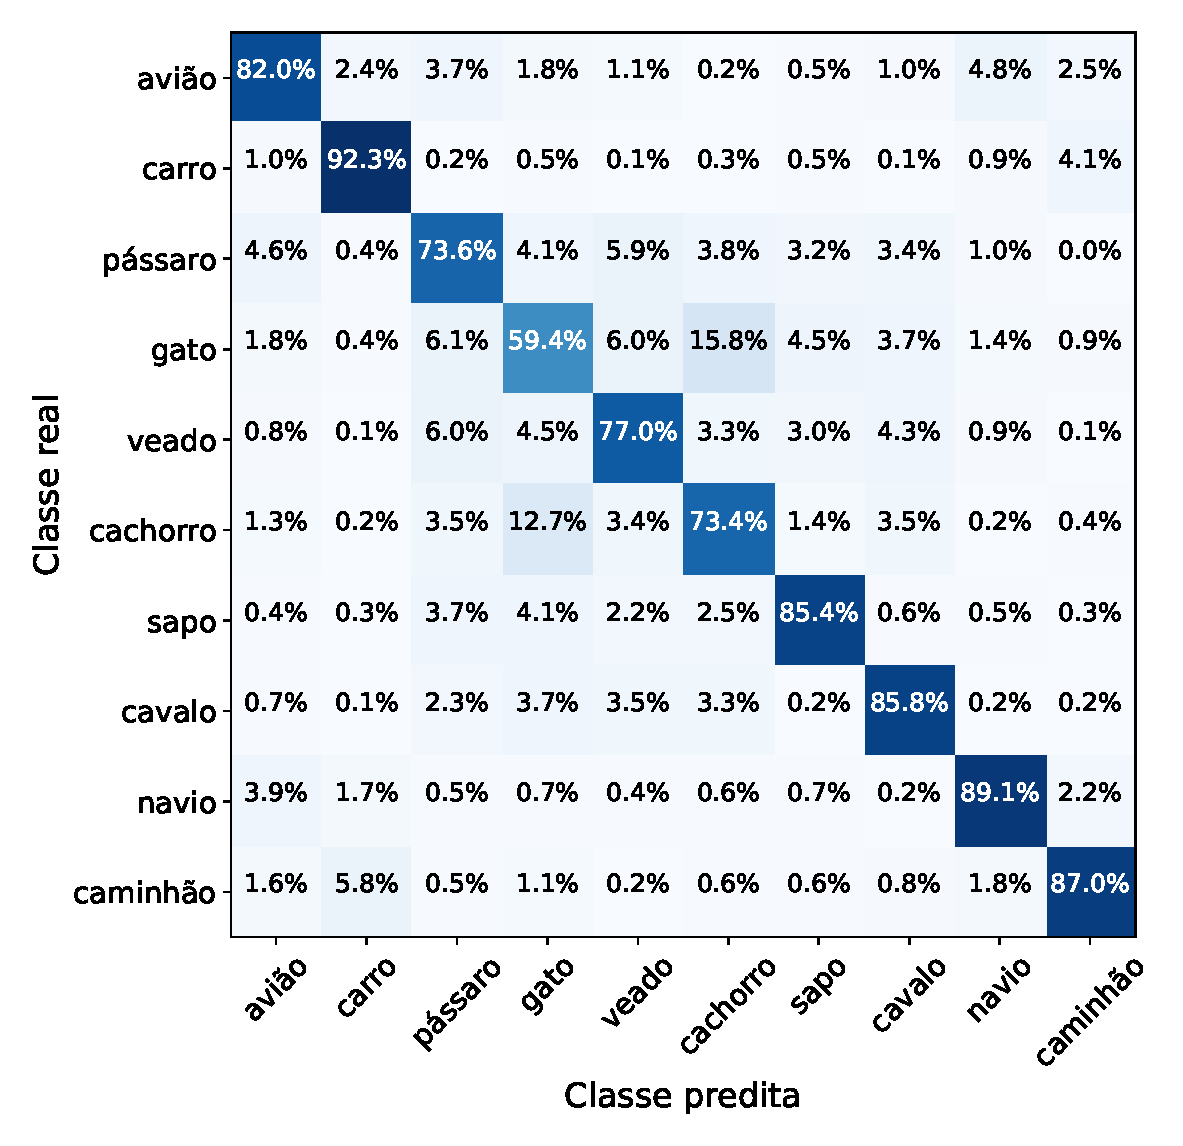
\includegraphics[width=\textwidth]{figuras/cifar_no_compress.eps}
          \caption{Modelo não comprimido}
        \end{subfigure}
        \hfill
        \begin{subfigure}[b]{0.49\textwidth}
          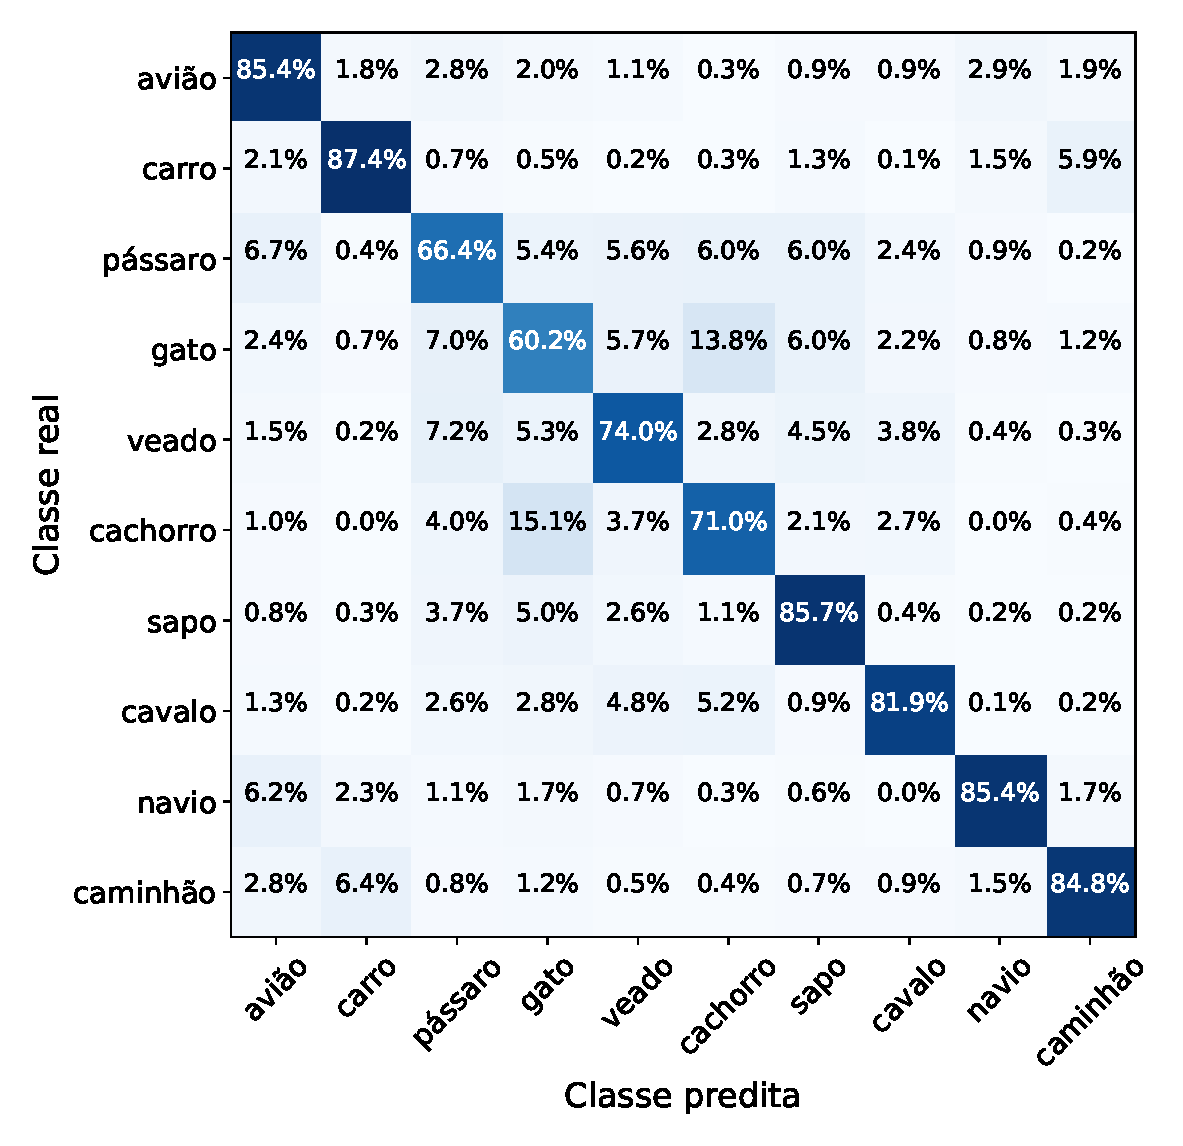
\includegraphics[width=\textwidth]{figuras/cifar_q8_p75.eps}
          \caption{8 bits e $\alpha = 1,25$}
        \end{subfigure}
        \caption{Matrizes de confusão do modelo sem compressão e do mais comprimido.}
    \end{figure}
\end{frame}


\begin{frame}{Resultados do treinamento}
    \begin{table}[H]
        \caption{Tamanho do modelo comprimido para vários valores de quantidade de bits e $\alpha$ em MegaBytes após compressão por Deflate}
        \centering
        \begin{tabular}{l|llll}
        \hline
        \textbf{\diagbox{bits}{$\alpha$}} & \textbf{0,00}  & \textbf{0,50} & \textbf{1,50} & \textbf{1,25}\\ \hline
        \textbf{32 bits} & 123,51MB	& 87,11MB & 55,80MB & 39,39MB\\
        \textbf{8 bits} & 32,50MB & 32,12MB & 22,09MB & 16,20MB\\\hline
        \end{tabular}
        \end{table}
\end{frame}

\begin{frame}{Resultados do treinamento}
    \begin{figure}[H]
        \centering
        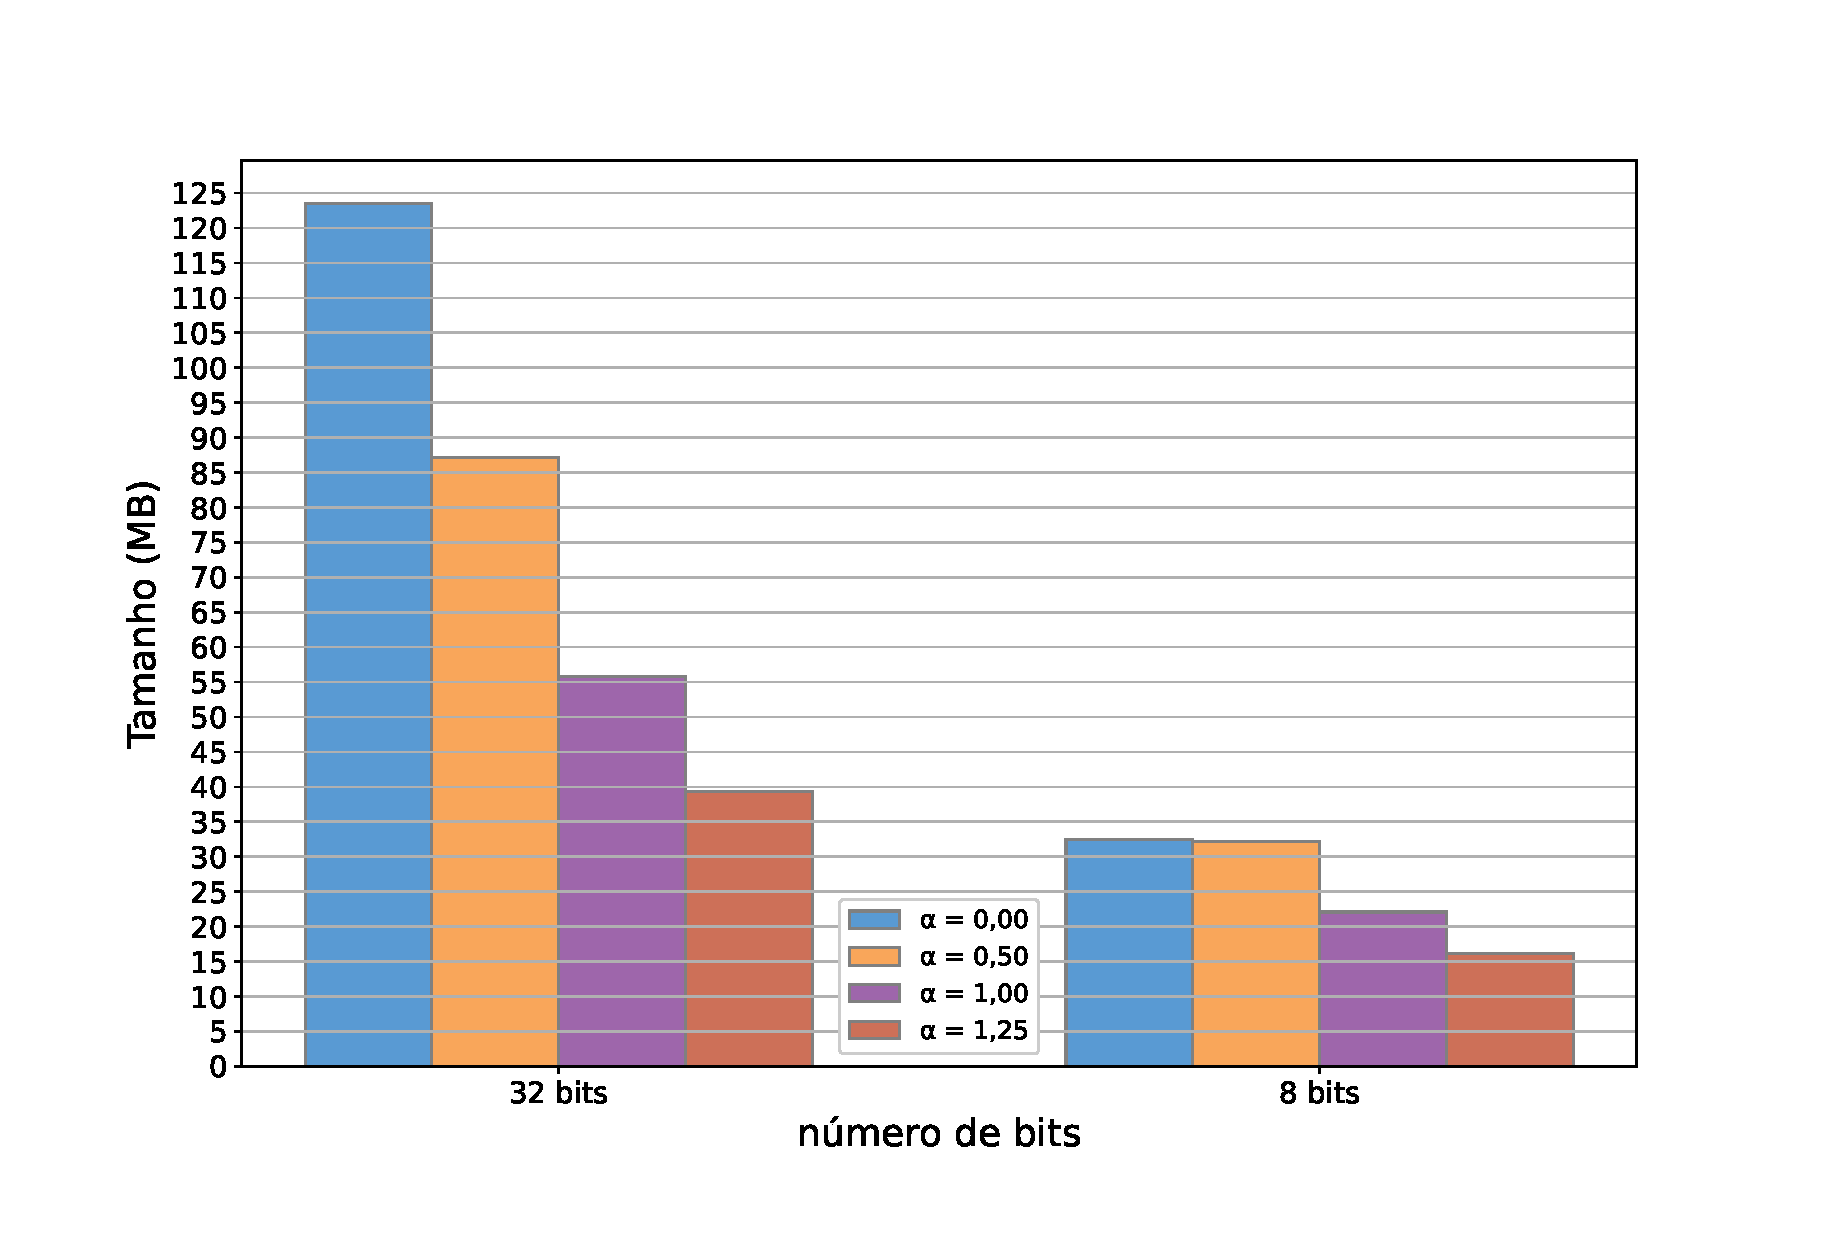
\includegraphics[width=0.7\textwidth]{figuras/cifar_mb_size_fig.eps}
        \caption{Tamanho do modelo comprimido para vários valores de quantidade de bits e $\alpha$ em MegaBytes após compressão por Deflate}
        \end{figure}
\end{frame}

\begin{frame}{Infraestrutura}
    \begin{figure}[H]
    \centering
    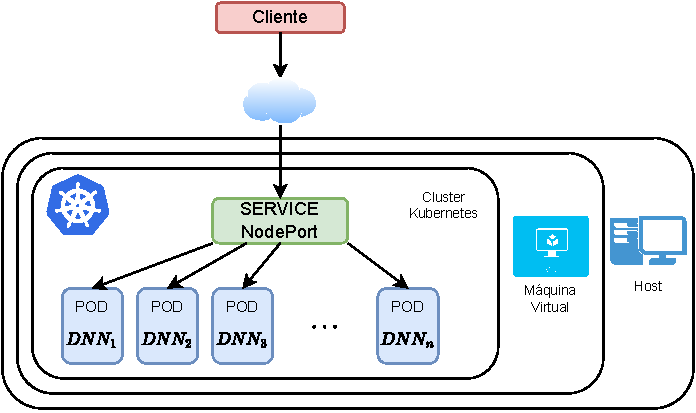
\includegraphics[width=0.7\textwidth]{figuras/infra.pdf}
    \caption{Infraestrutura geral desenvolvida}
    \end{figure}
\end{frame}

\begin{frame}{Configurações dos pods}
    Cada pod foi construído com as seguintes características:
    \begin{itemize}
        \item Máximo de processamento em 100miliCPU;
        \item Nova réplica com 20\% do máximo de processamento;
        \item Máximo de 10 réplicas.
    \end{itemize}
\end{frame}

\begin{frame}{Perfil de estresse}
    Foram criados perfis de estresse utilizando o \textit{Open Model Thread Group} da ferramenta Apache JMeter, para variar a quantidade de requisições do sistema com o passar do tempo.
    \begin{figure}[H]
    \centering
    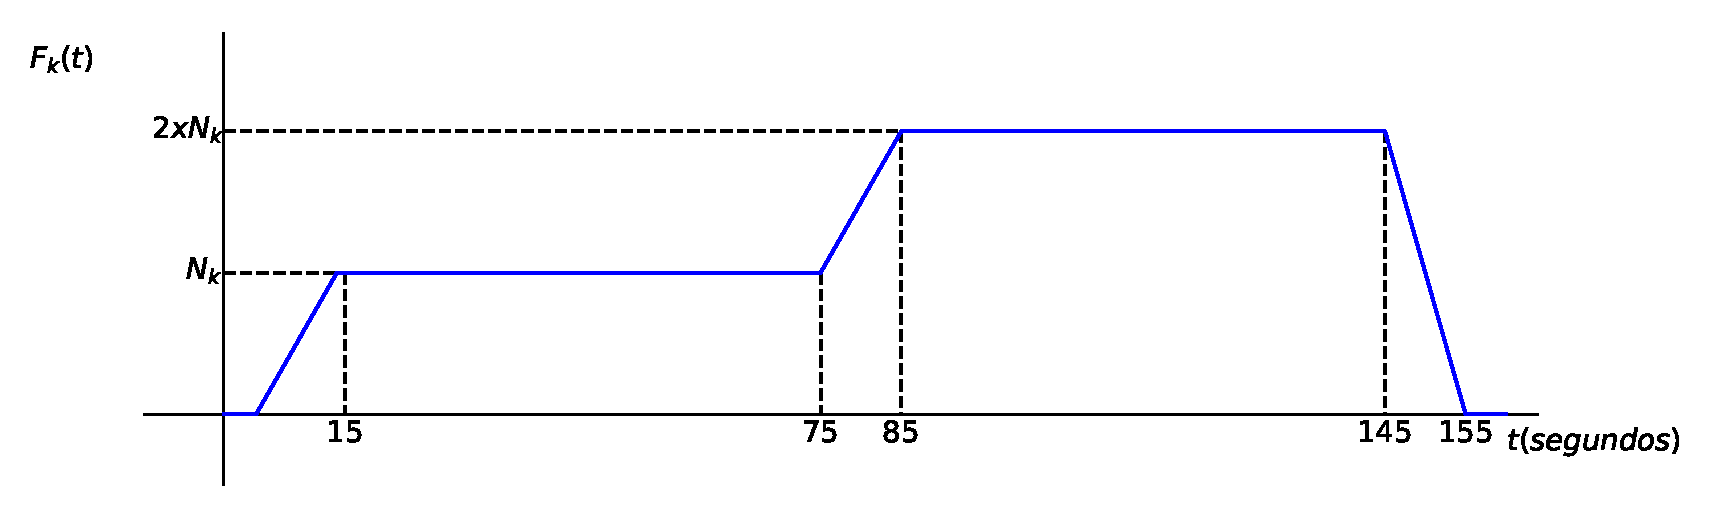
\includegraphics[width=1\textwidth]{figuras/estresse.eps}
    \caption{Perfil de estresse com $n$ variando em $75$, $125$ e $250$}
    \end{figure}
\end{frame}

\begin{frame}{Resultados}
    \scriptsize
    \begin{table}[H]
        \caption{\scriptsize{Latência de resposta das requisições, Consumo de memória e processamento de cada microseriviço do primeiro perfil de estresse $N_1 = 75$.}}
        \centering
        \begin{tabular}{llllll} \\
        \hline
        \textbf{bits} & \textbf{$\alpha$}  &  \textbf{Latência} & \textbf{Memória} &\textbf{CPU}\\  \hline
        32 &0,00& $16,23ms \pm 2,988$ & 701MiB & 135miliCPU\\
        32 &0,50& $15,97ms \pm 3,467$ & 707MiB & 136miliCPU\\
        32 &1,00& $16,02ms \pm 2,659$ & 701MiB & 143miliCPU\\
        32 &1,25& $15,44ms \pm 2,597$ & 703MiB & 132miliCPU\\
        8  &0,00& $9,39ms \pm 2,026$ & 412MiB & 95miliCPU\\
        8  &0,50& $9,27ms \pm 3,011$ & 414MiB & 94miliCPU\\
        8  &1,00& $9,57ms \pm 2,144$ & 411MiB & 96miliCPU\\
        8  &1,25& $9,44ms \pm 1,729$ & 411MiB & 94miliCPU\\
        \hline
        \end{tabular}
        \end{table}
\end{frame}

\begin{frame}{Resultados}
    \begin{figure}[H]
        \centering
        \begin{subfigure}[b]{0.32\textwidth}
            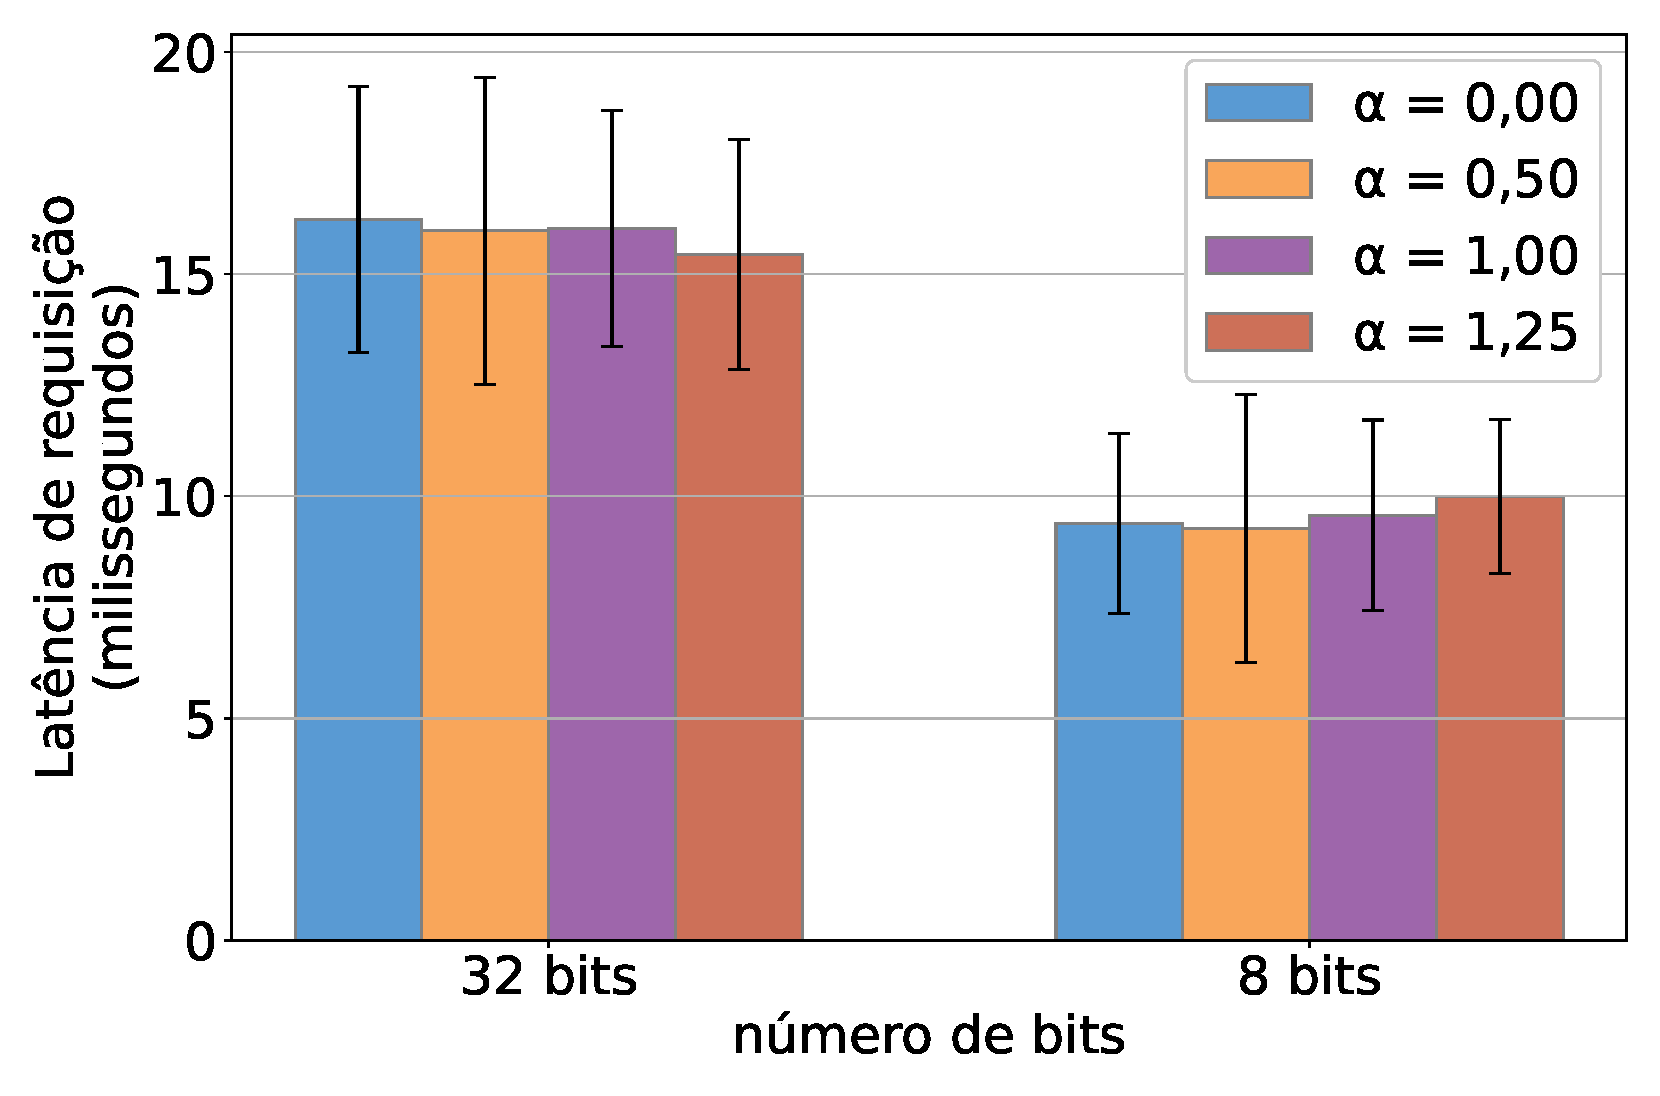
\includegraphics[width=\textwidth]{figuras/latencia1.eps}
            \caption{\scriptsize{Latências}}
          \end{subfigure}  
          \begin{subfigure}[b]{0.32\textwidth}
            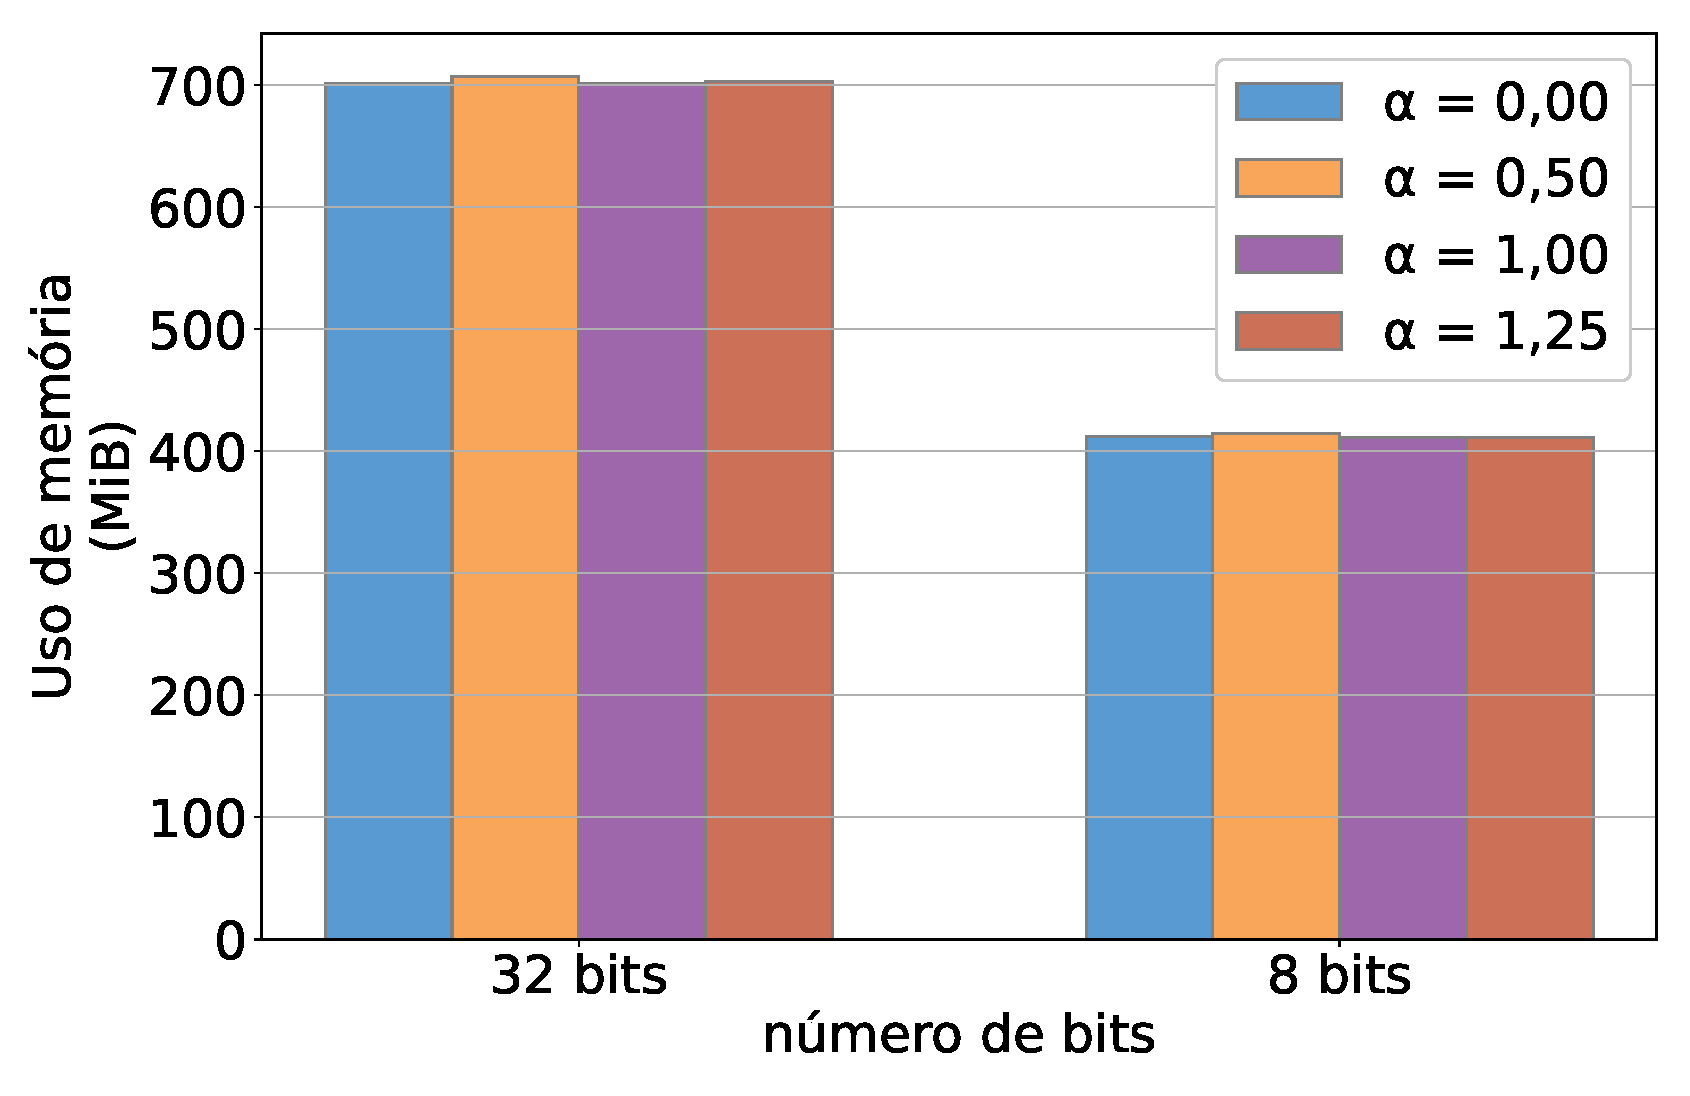
\includegraphics[width=\textwidth]{figuras/memoria1.eps}
            \caption{\scriptsize{Consumo de memória}}
        \end{subfigure}
        \begin{subfigure}[b]{0.32\textwidth}
            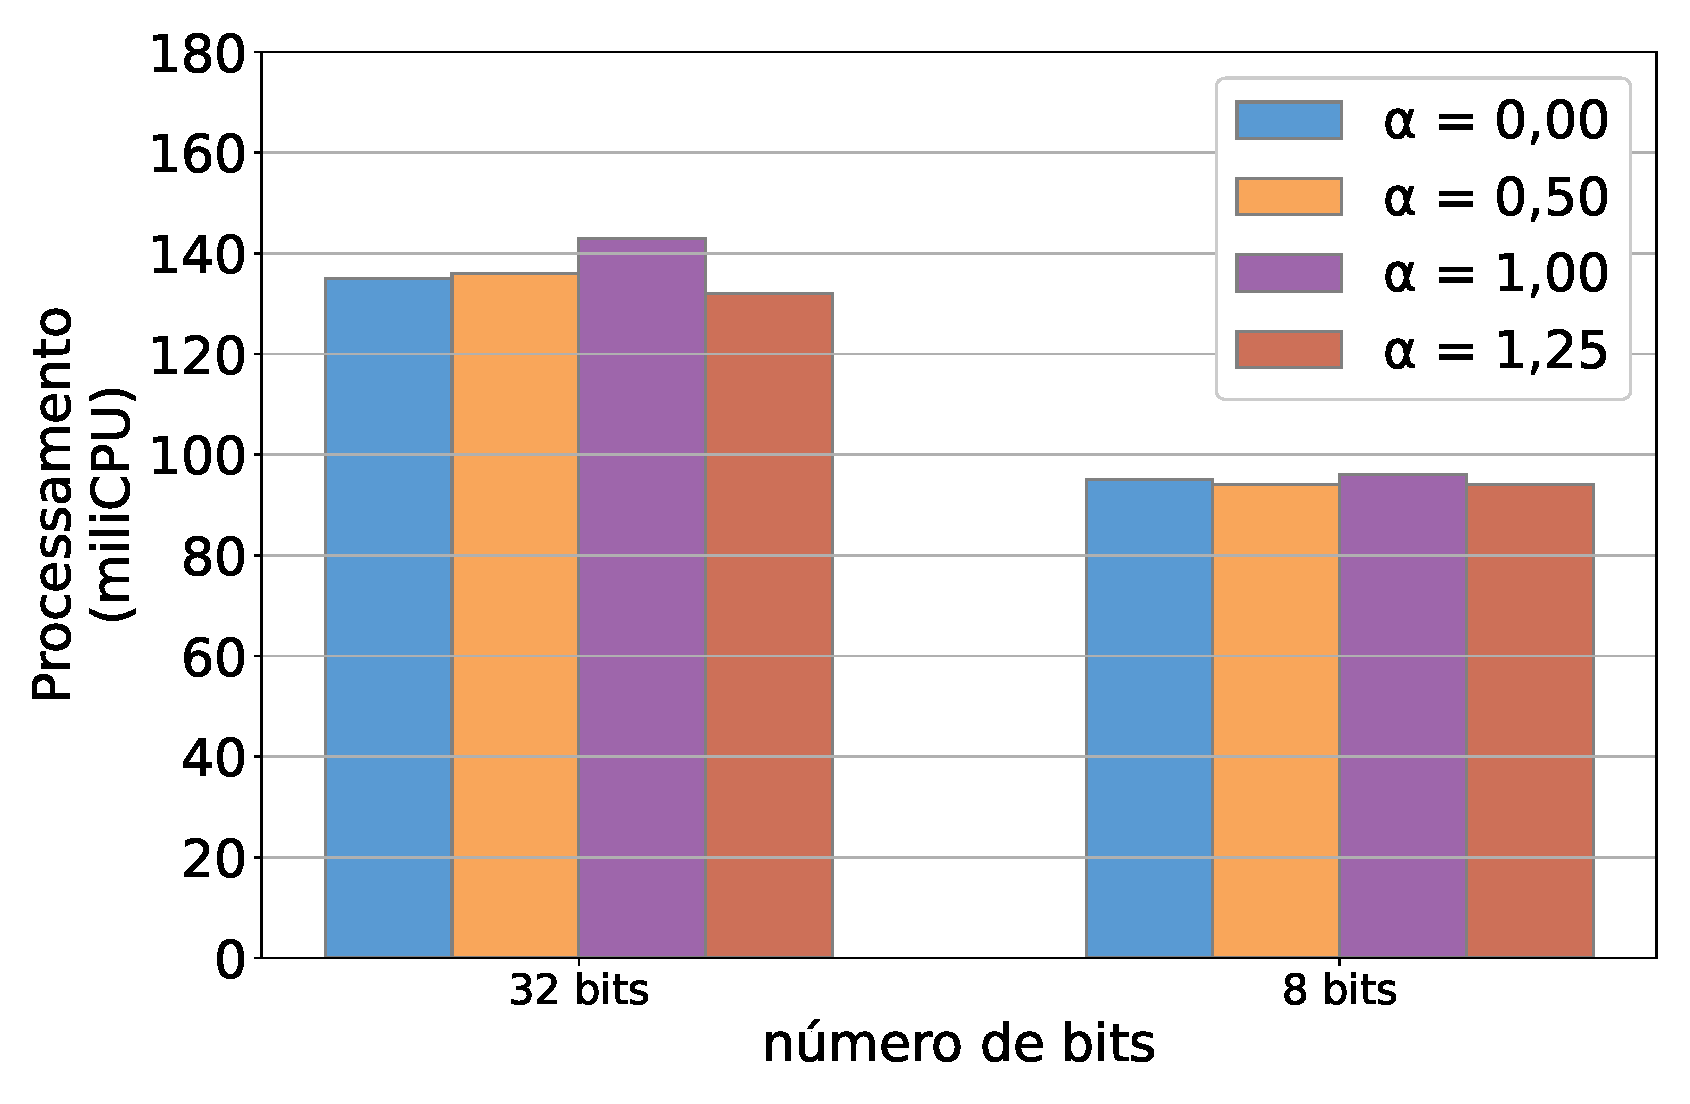
\includegraphics[width=\textwidth]{figuras/cpu1.eps}
            \caption{\scriptsize{Processamento}}
        \end{subfigure}
        \caption{\scriptsize{Latência de resposta em milissegundos, consumo de memória e uso de CPU de cada microserviço para o primeiro perfil de estresse $N_1 = 75$.}}
        \end{figure}
\end{frame}


\begin{frame}{Resultados}
    \scriptsize
    \begin{table}[H]
        \caption{\scriptsize{Latência de resposta das requisições, Consumo de memória e processamento de cada microseriviço do segundo perfil de estresse $N_2 = 125$.}}
        \centering
        \begin{tabular}{llllll} \\
        \hline
        \textbf{bits} & \textbf{$\alpha$}  &  \textbf{Latência} & \textbf{Memória} &\textbf{CPU}\\  \hline
        32 &0,00& $16,01ms \pm 2,755$ & 701MiB & 136miliCPU\\
        32 &0,50& $16,44ms \pm 3,134$ & 704MiB & 137miliCPU\\
        32 &1,00& $15,51ms \pm 2,299$ & 703MiB & 139miliCPU\\
        32 &1,25& $15,23ms \pm 3,101$ & 703MiB & 136miliCPU\\
        8  &0,00& $9,22ms \pm 2,577$ & 411MiB & 94miliCPU\\
        8  &0,50& $8,68ms \pm 3,822$ & 412MiB & 94miliCPU\\
        8  &1,00& $8,67ms \pm 3,715$ & 411MiB & 95miliCPU\\
        8  &1,25& $9,58ms \pm 3,122$ & 411MiB & 94miliCPU\\
        \hline
        \end{tabular}
        \end{table}
\end{frame}

\begin{frame}{Resultados}
    \begin{figure}[H]
        \centering
        \begin{subfigure}[b]{0.32\textwidth}
            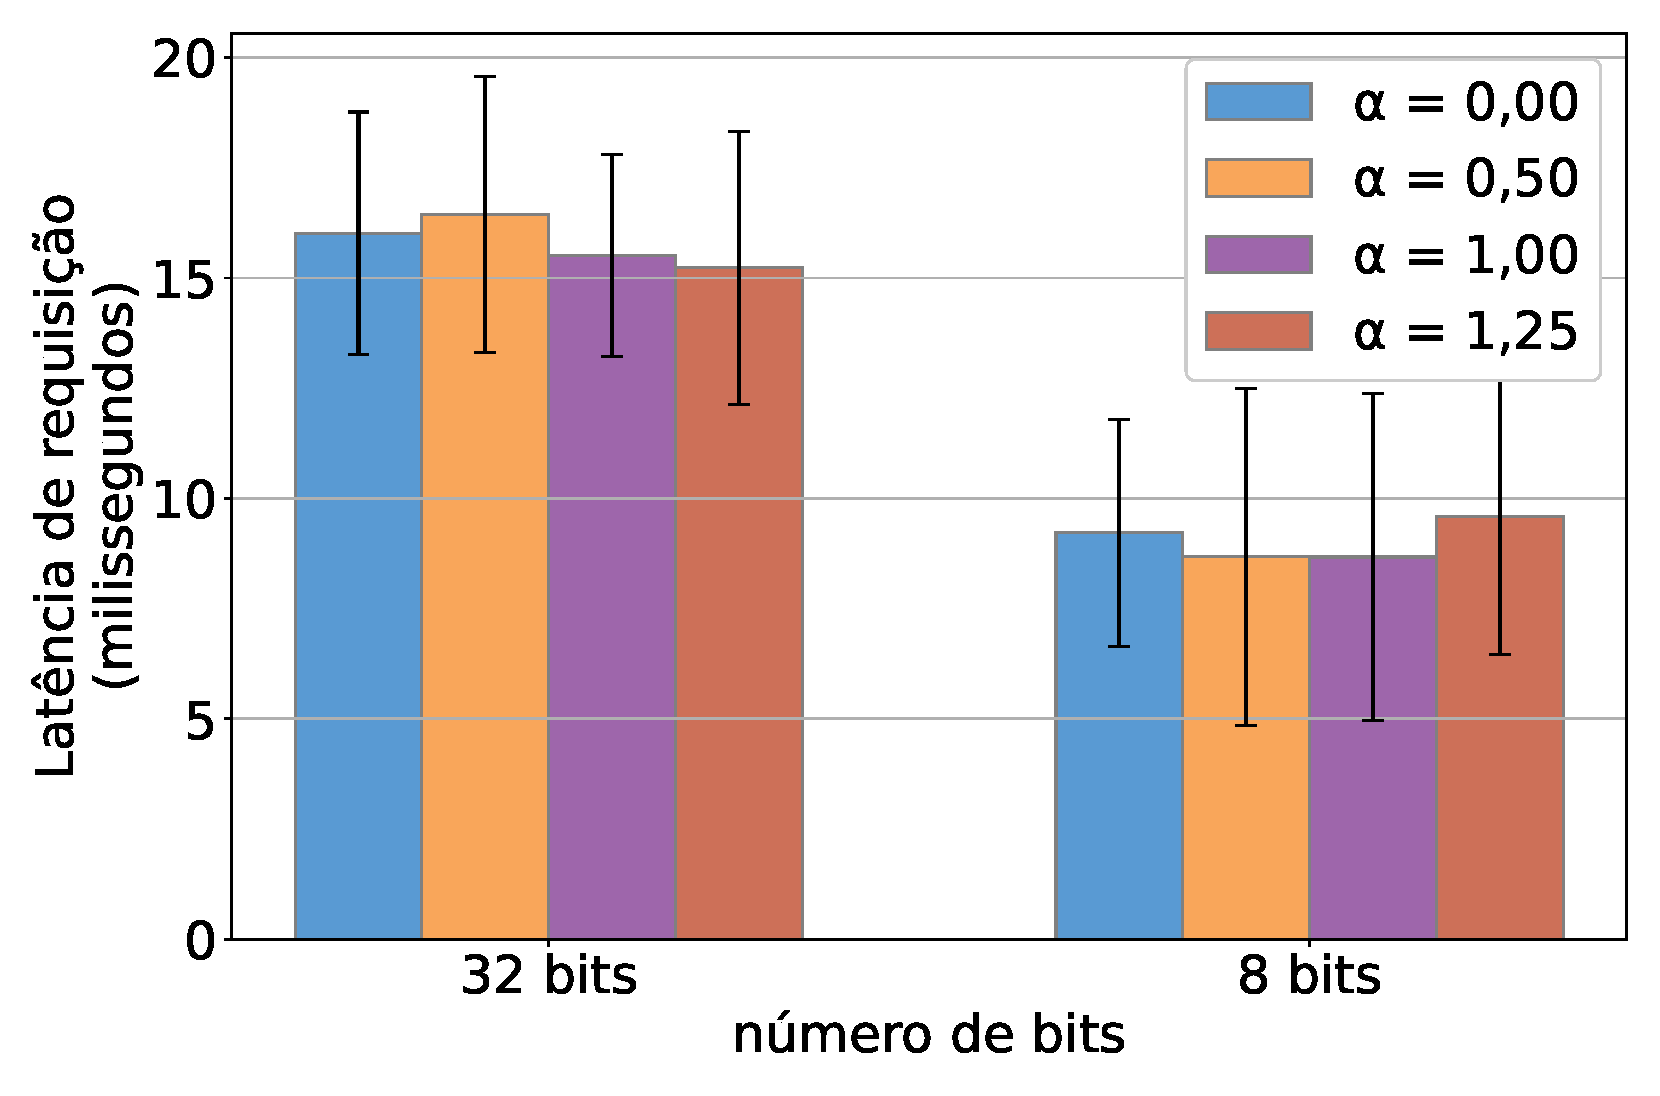
\includegraphics[width=\textwidth]{figuras/latencia2.eps}
            \caption{\scriptsize{Latências}}
          \end{subfigure}  
          \begin{subfigure}[b]{0.32\textwidth}
            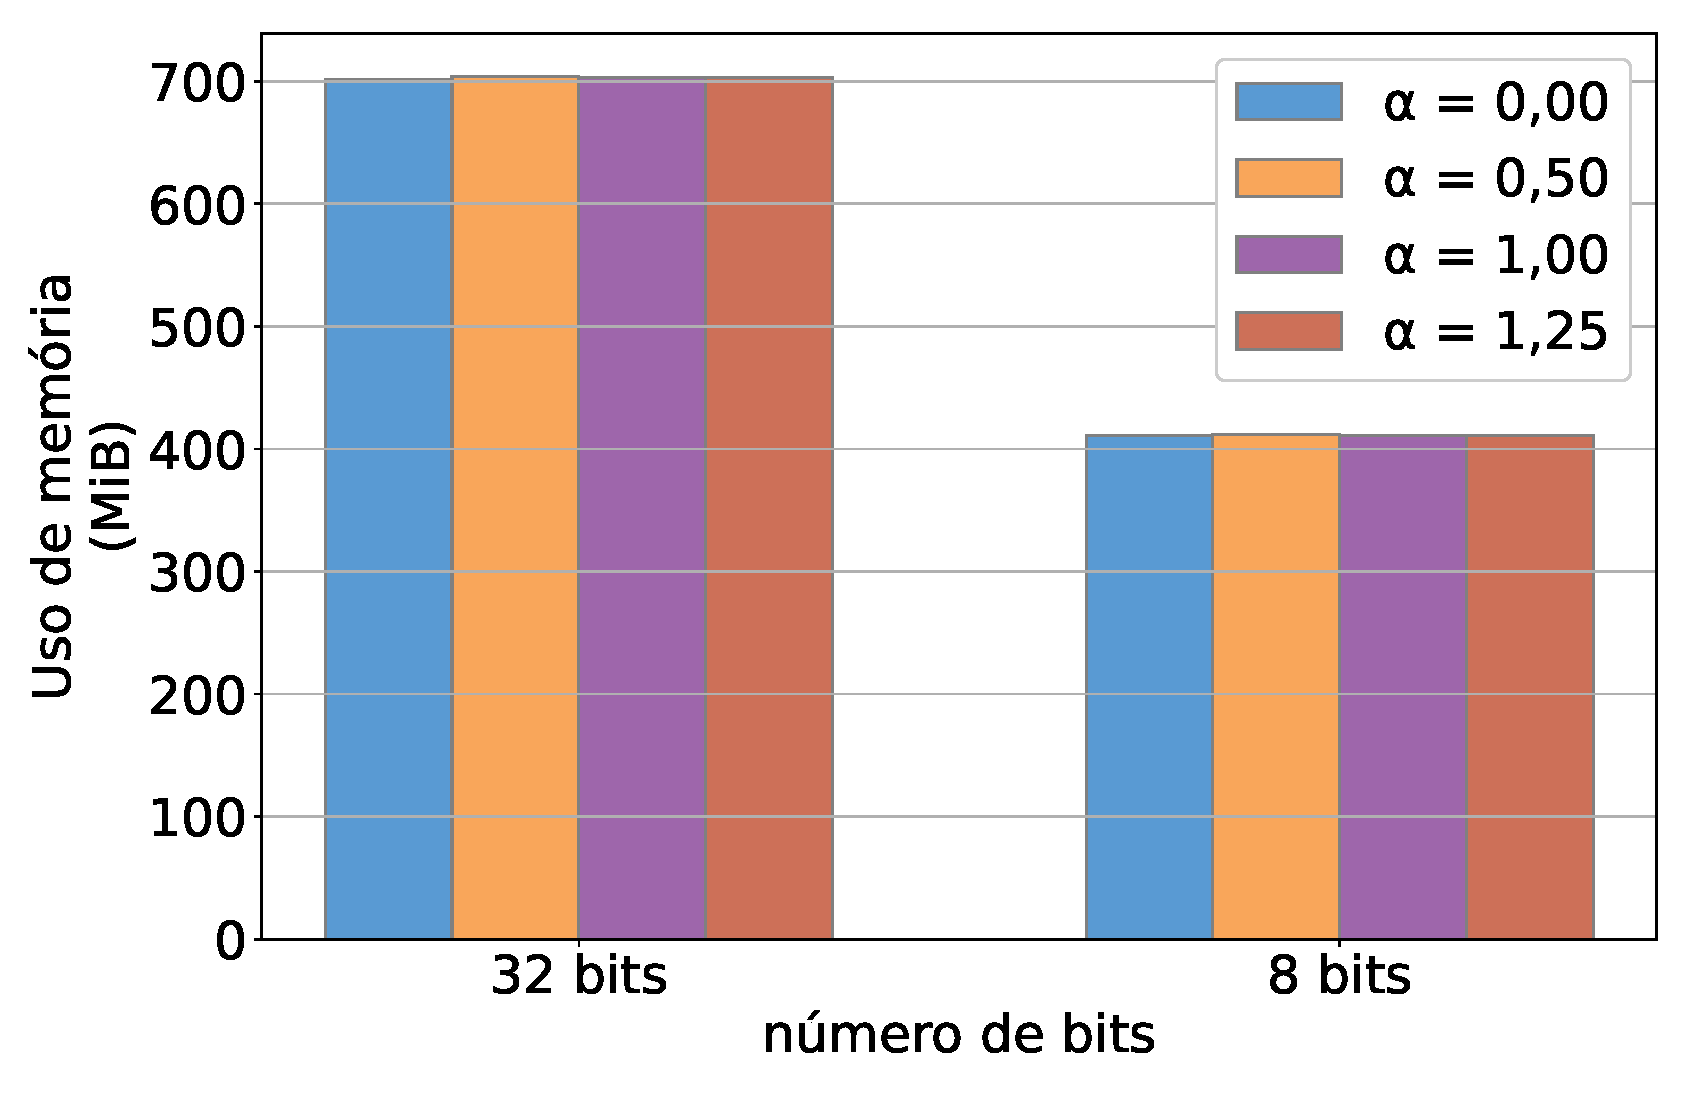
\includegraphics[width=\textwidth]{figuras/memoria2.eps}
            \caption{\scriptsize{Consumo de memória}}
        \end{subfigure}
        \begin{subfigure}[b]{0.32\textwidth}
            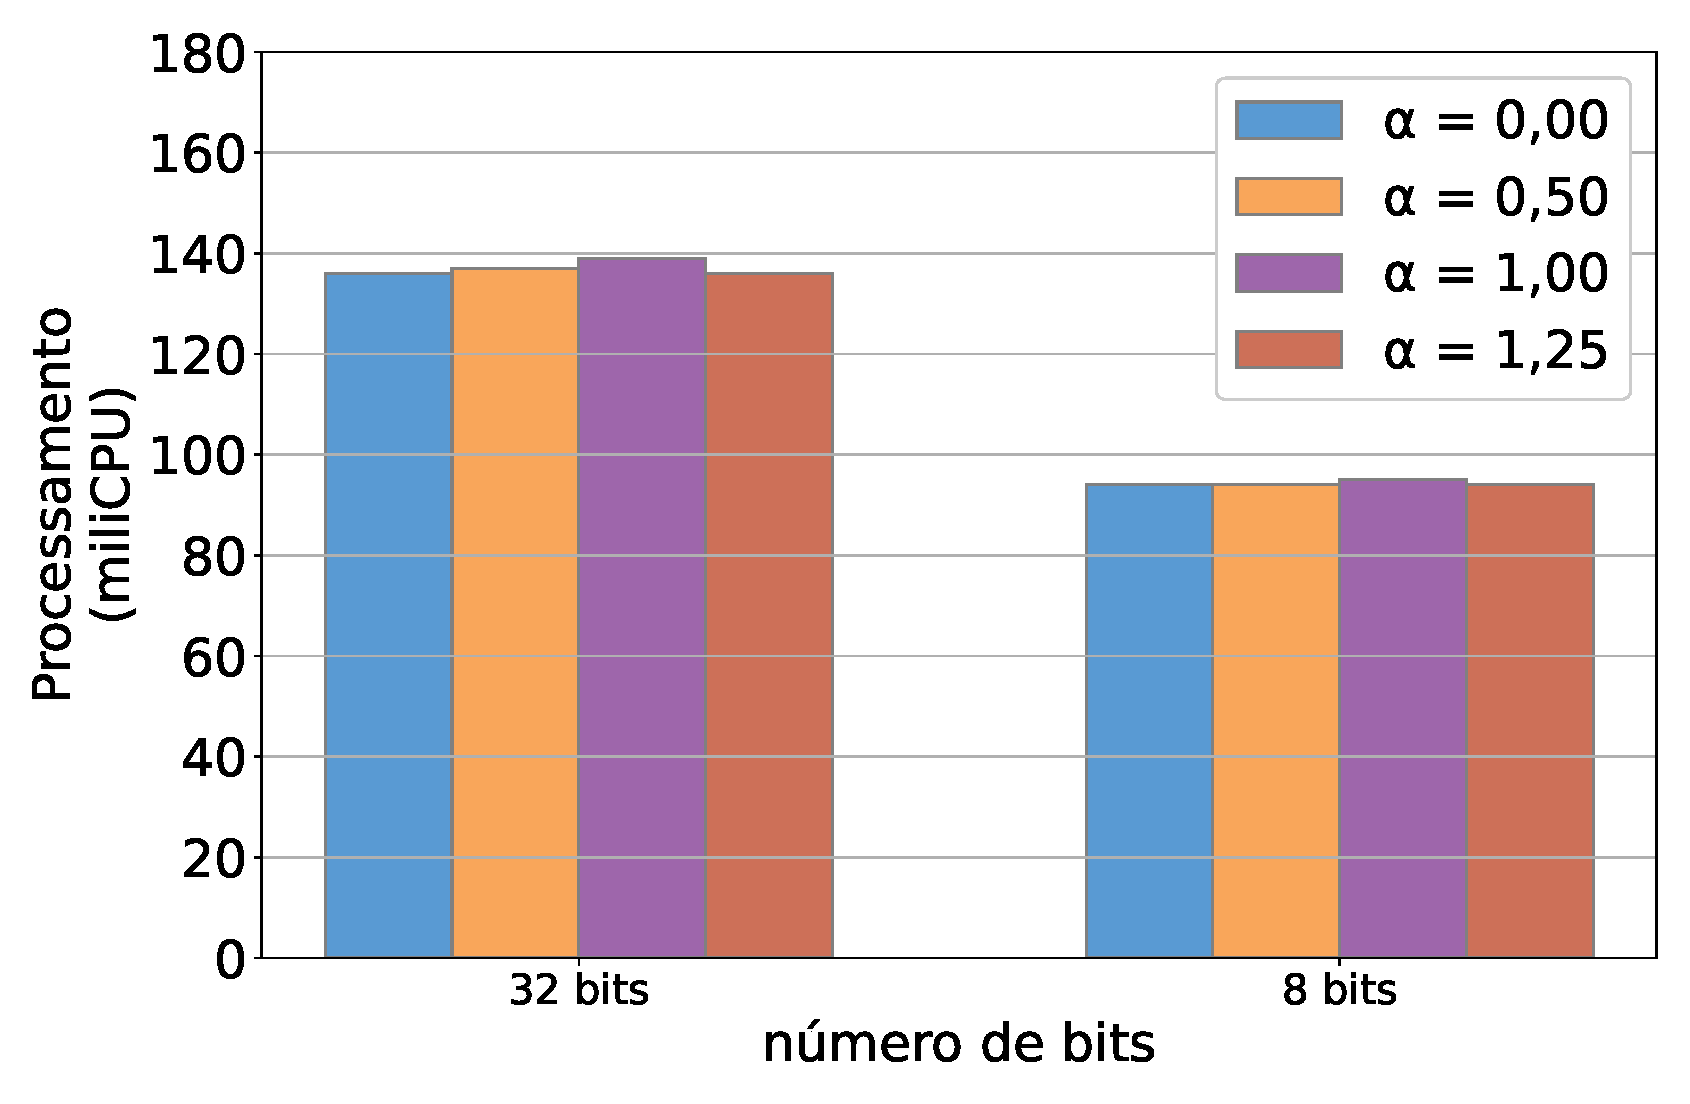
\includegraphics[width=\textwidth]{figuras/cpu2.eps}
            \caption{\scriptsize{Processamento}}
        \end{subfigure}
        \caption{\scriptsize{Latência de resposta em milissegundos, consumo de memória e uso de CPU de cada microserviço para o segundo perfil de estresse $N_2 = 125$.}}
        \end{figure}
\end{frame}

\begin{frame}{Resultados}
    \scriptsize
    \begin{table}[H]
        \caption{\scriptsize{Latência de resposta das requisições, Consumo de memória e processamento de cada microseriviço do terceiro perfil de estresse $N_3 = 250$.}}
        \centering
        \begin{tabular}{llllll} \\
        \hline
        \textbf{bits} & \textbf{$\alpha$}  &  \textbf{Latência} & \textbf{Memória} &\textbf{CPU}\\  \hline
        32 &0,00& $16,23ms \pm 3,122$ & 702MiB & 135miliCPU\\
        32 &0,50& $16,78ms \pm 3,214$ & 706MiB & 136miliCPU\\
        32 &1,00& $16,24ms \pm 3,333$ & 704MiB & 139miliCPU\\
        32 &1,25& $15,34ms \pm 2,767$ & 701MiB & 134miliCPU\\
        8  &0,00& $9,30ms \pm 2,666$ & 412MiB & 94miliCPU\\
        8  &0,50& $9,25ms \pm 2,714$ & 414MiB & 95miliCPU\\
        8  &1,00& $9,25ms \pm 2,555$ & 410MiB & 96miliCPU\\
        8  &1,25& $8,71ms \pm 2,991$ & 411MiB & 94miliCPU\\
        \hline
        \end{tabular}
        \end{table}
\end{frame}

\begin{frame}{Resultados}
    \begin{figure}[H]
        \centering
        \begin{subfigure}[b]{0.32\textwidth}
            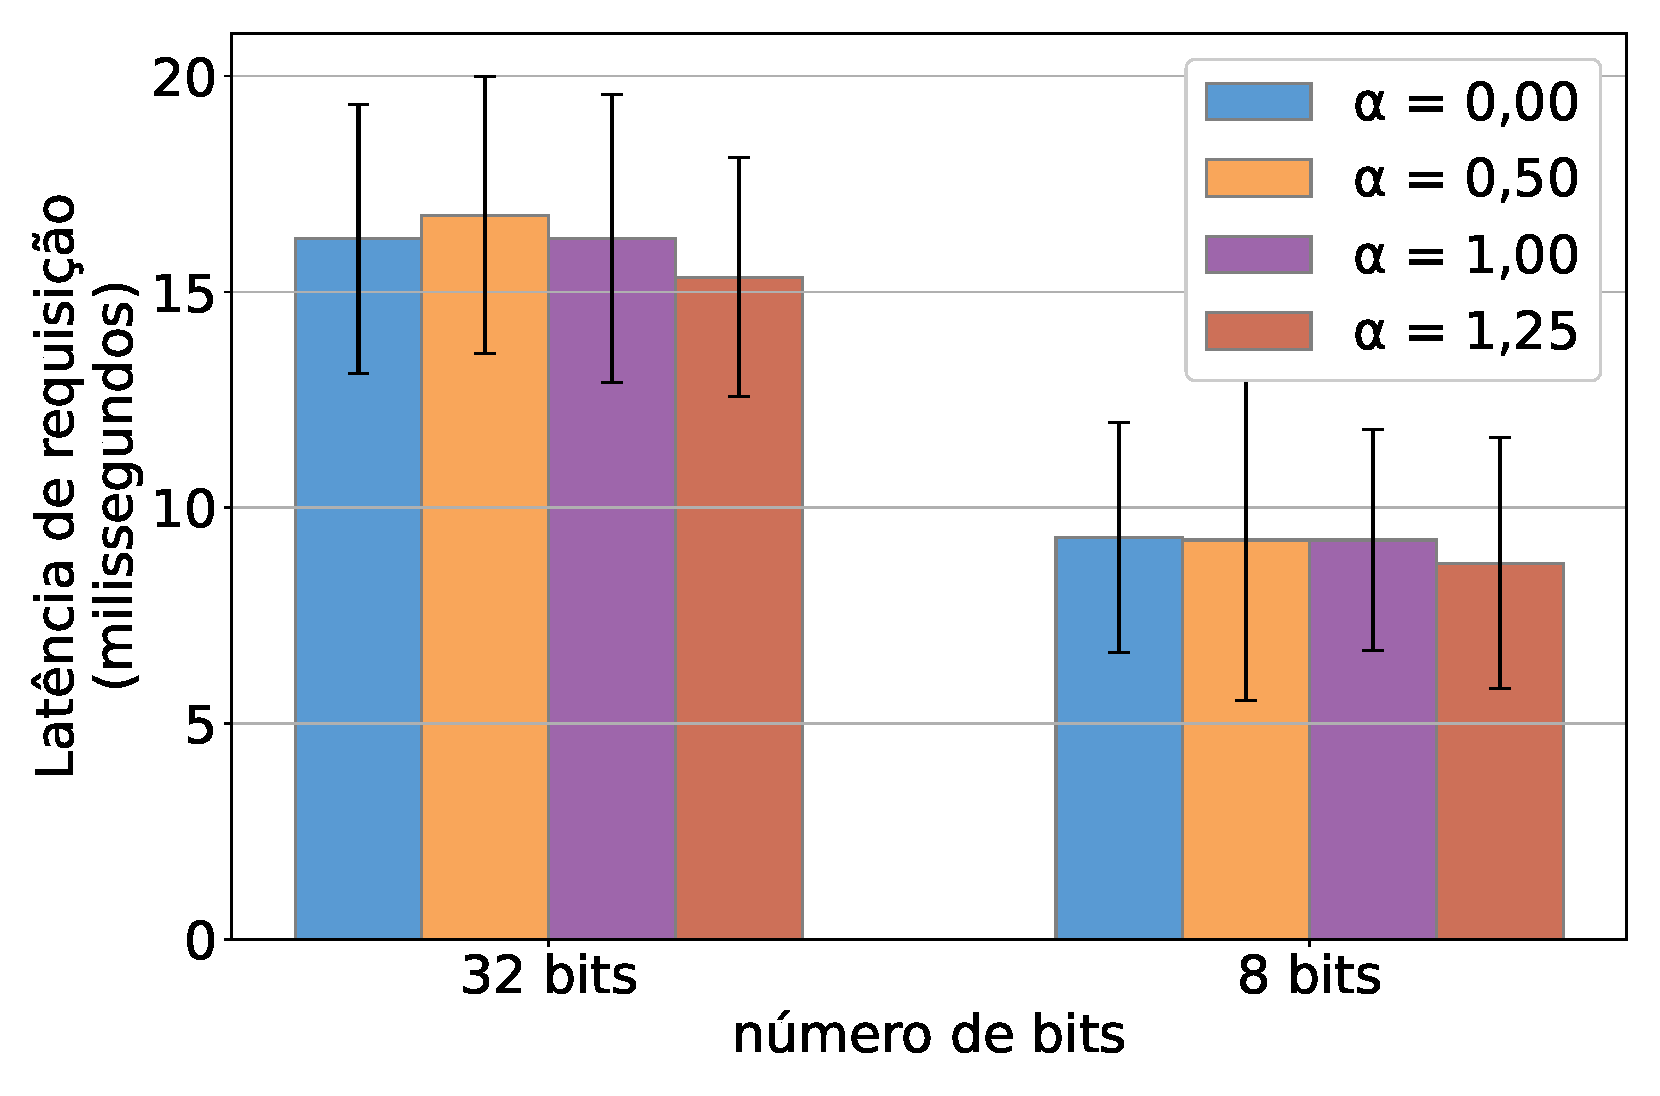
\includegraphics[width=\textwidth]{figuras/latencia3.eps}
            \caption{\scriptsize{Latências}}
          \end{subfigure}  
          \begin{subfigure}[b]{0.32\textwidth}
            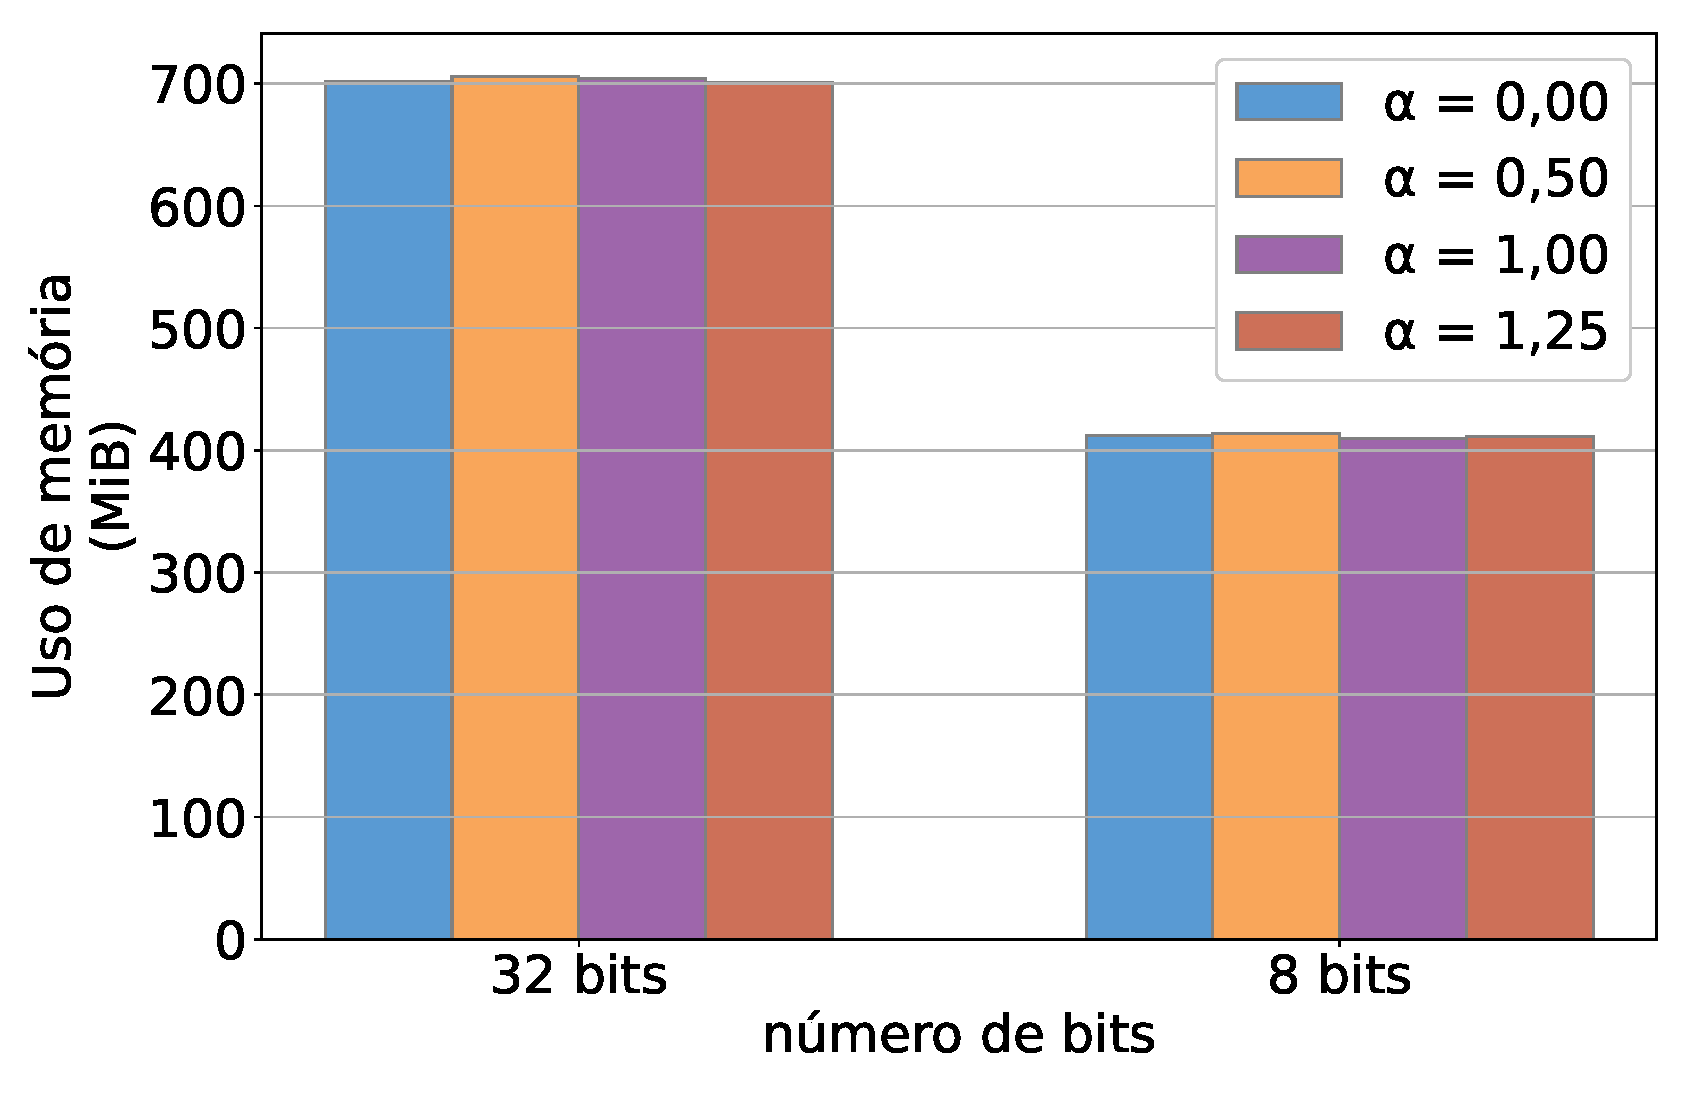
\includegraphics[width=\textwidth]{figuras/memoria3.eps}
            \caption{\scriptsize{Consumo de memória}}
        \end{subfigure}
        \begin{subfigure}[b]{0.32\textwidth}
            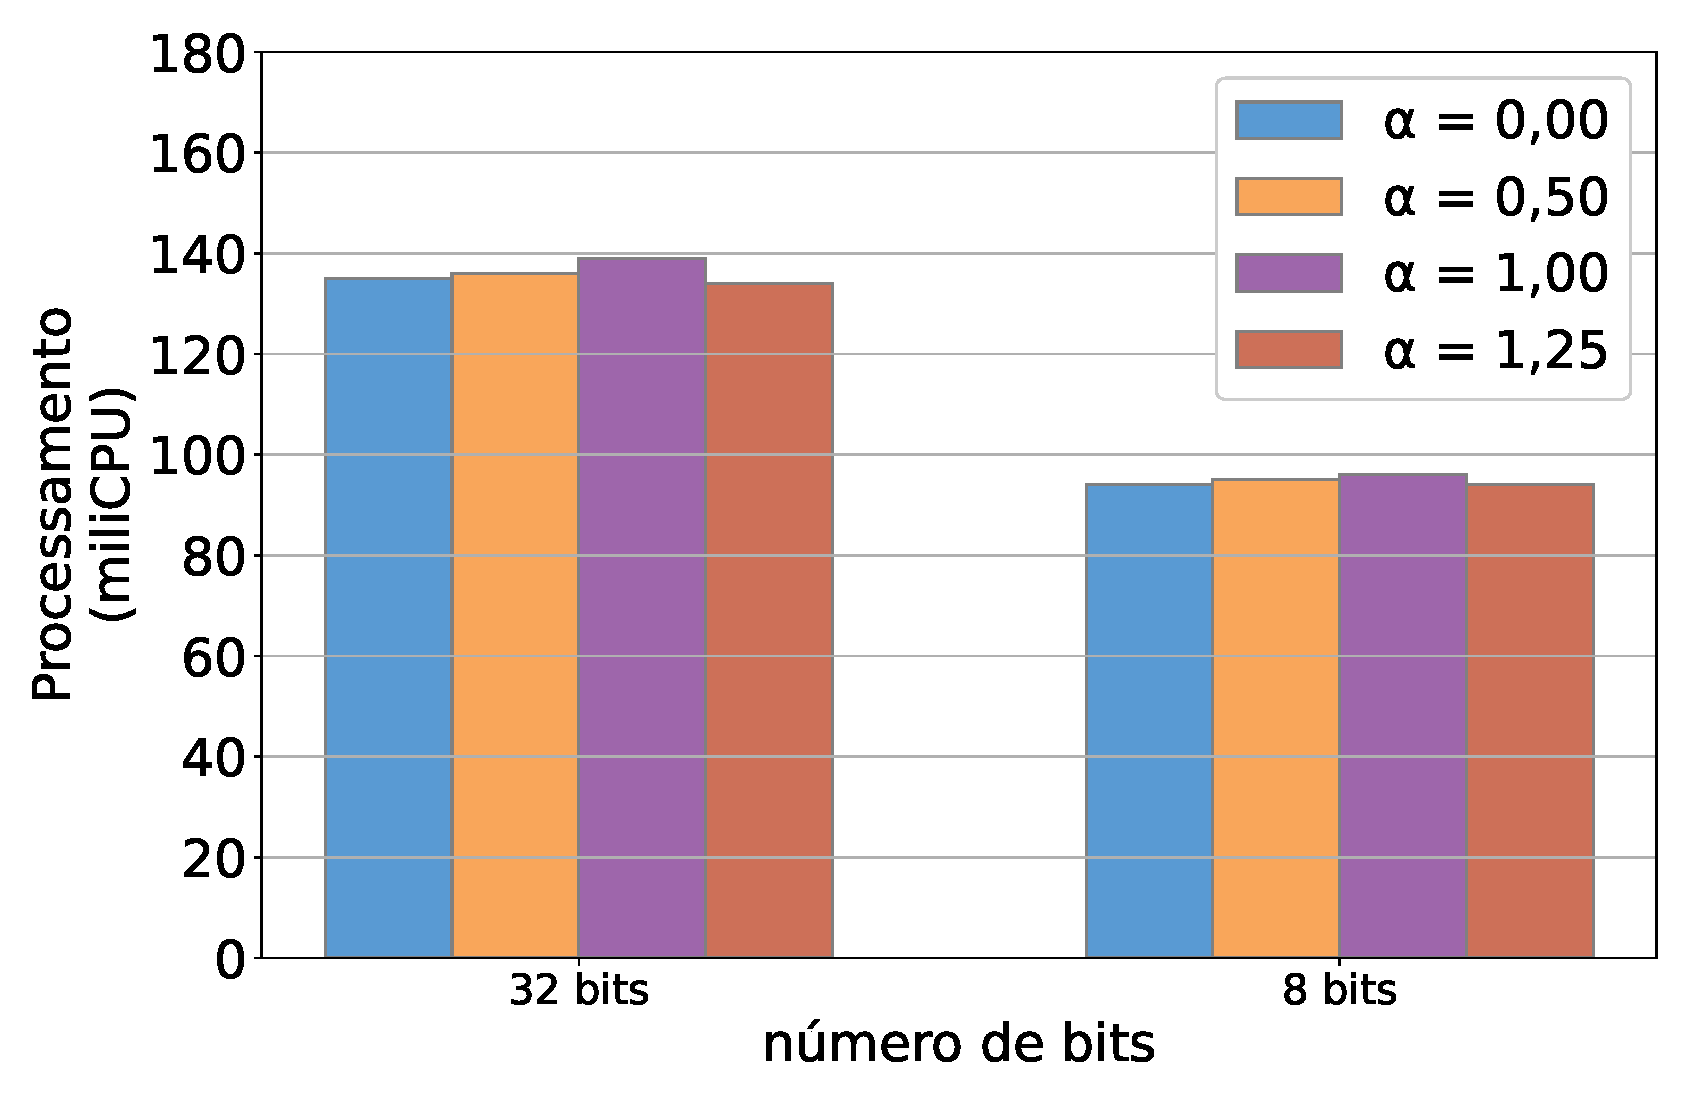
\includegraphics[width=\textwidth]{figuras/cpu3.eps}
            \caption{\scriptsize{Processamento}}
        \end{subfigure}
        \caption{\scriptsize{Latência de resposta em milissegundos, consumo de memória e uso de CPU de cada microserviço para o terceiro perfil de estresse $N_3 = 250$.}}
    \end{figure}
\end{frame}

\begin{frame}{Resultados}
    \scriptsize
    \begin{table}[H]
        \caption{\scriptsize{Tempo médio para criação de uma nova réplica.}}
        \centering
        \begin{tabular}{l|llll}
        \hline
        \textbf{\diagbox{bits}{$\alpha$}} & \textbf{0,00}  & \textbf{0,50} & \textbf{1,50} & \textbf{1,25}\\ \hline
        \textbf{32 bits} & $2,71s \pm 0,0220$ & $2,72s \pm 0,0267$ & $2,57s \pm 0,0306$ & $2,41s \pm 0,0294$\\
        \textbf{8 bits} & $2,30s \pm 0,0199$ & $2,25s \pm 0,0444$ & $2,22s \pm 0,0212$ & $2,14s \pm 0,0409$\\\hline
        \end{tabular}
    \end{table}
\end{frame}

\begin{frame}{Resultados}
    \begin{figure}[H]
        \centering
        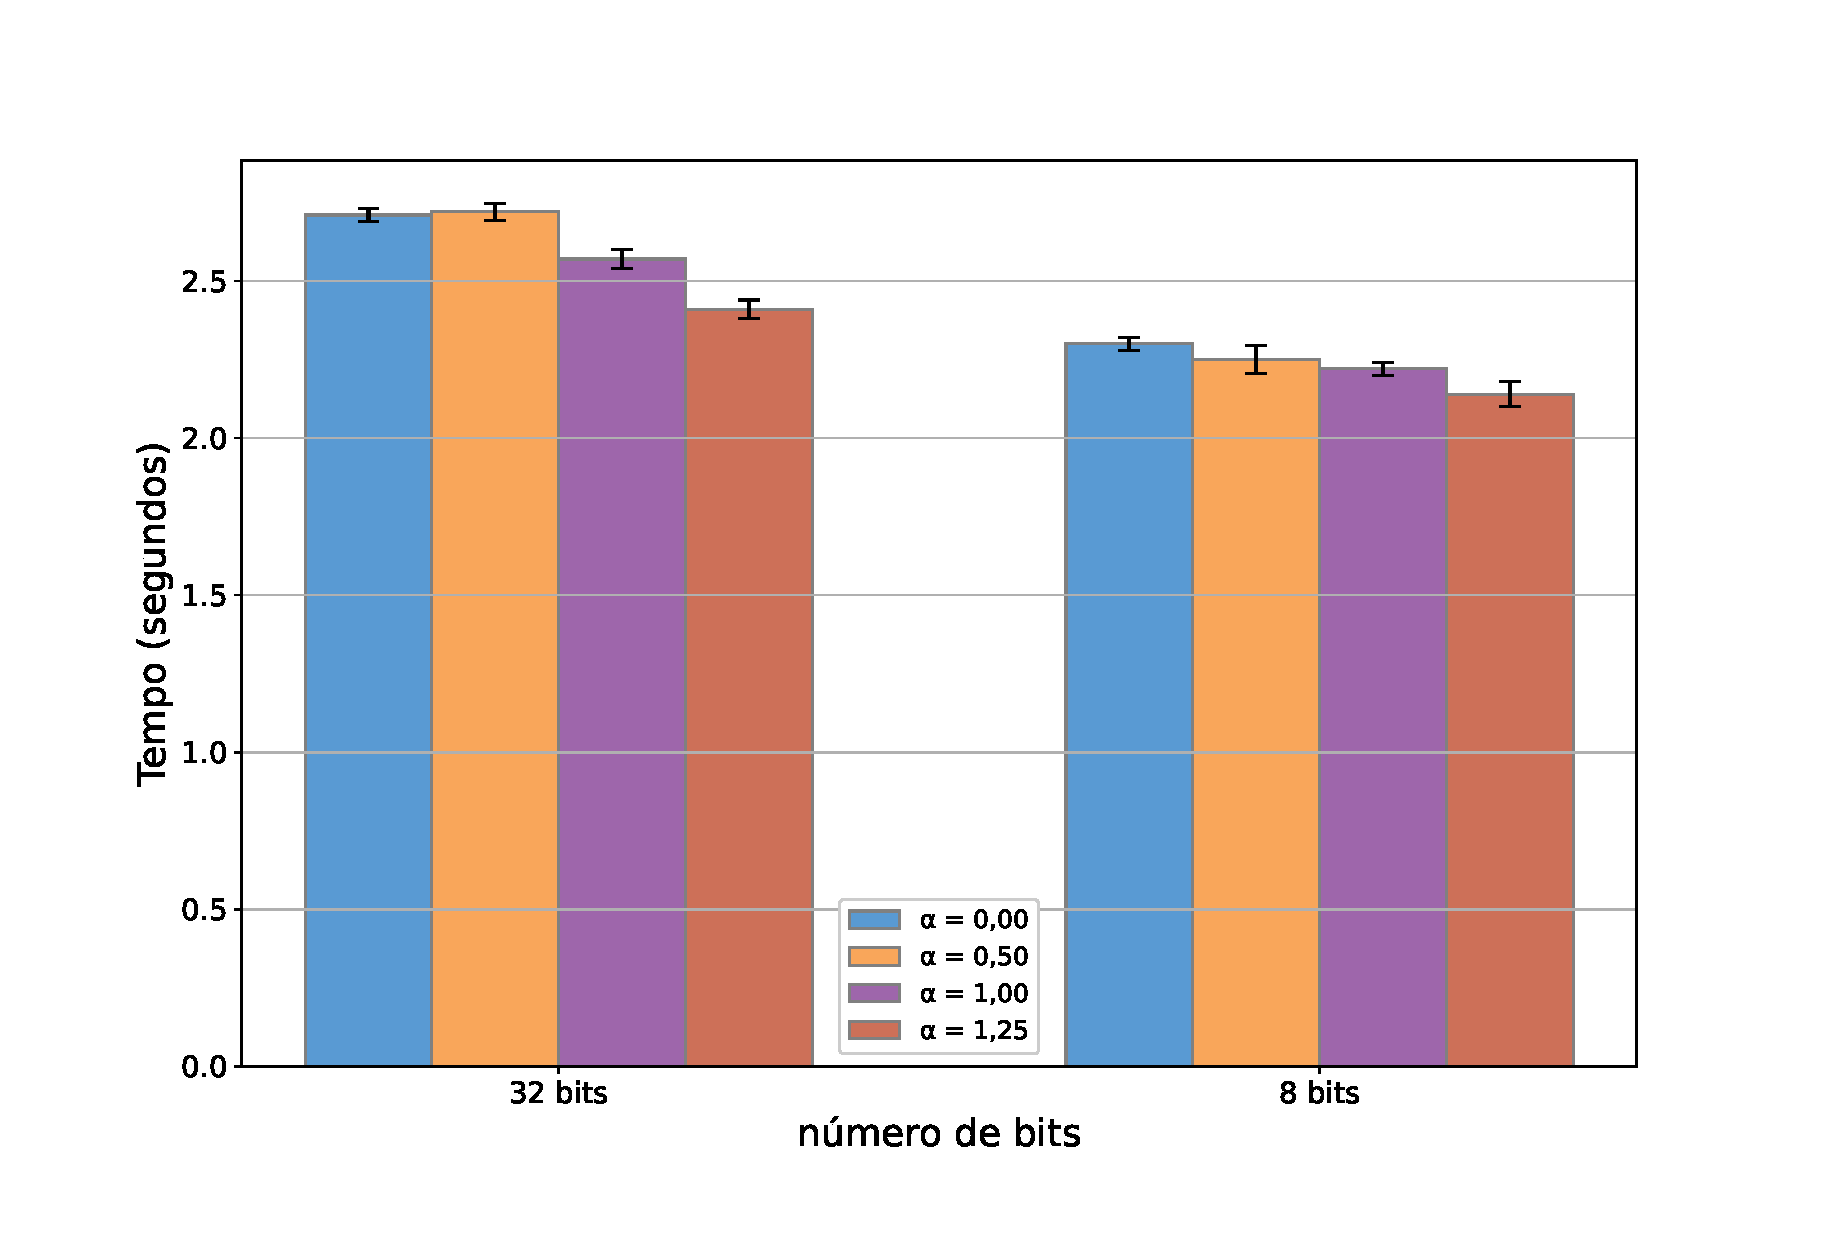
\includegraphics[width=0.7\textwidth]{figuras/hpa.eps}
        \caption{Tempo médio para criação de uma nova réplica.}
    \end{figure}
\end{frame}


\begin{frame}{Resultados}
    \begin{figure}[H]
    \centering
    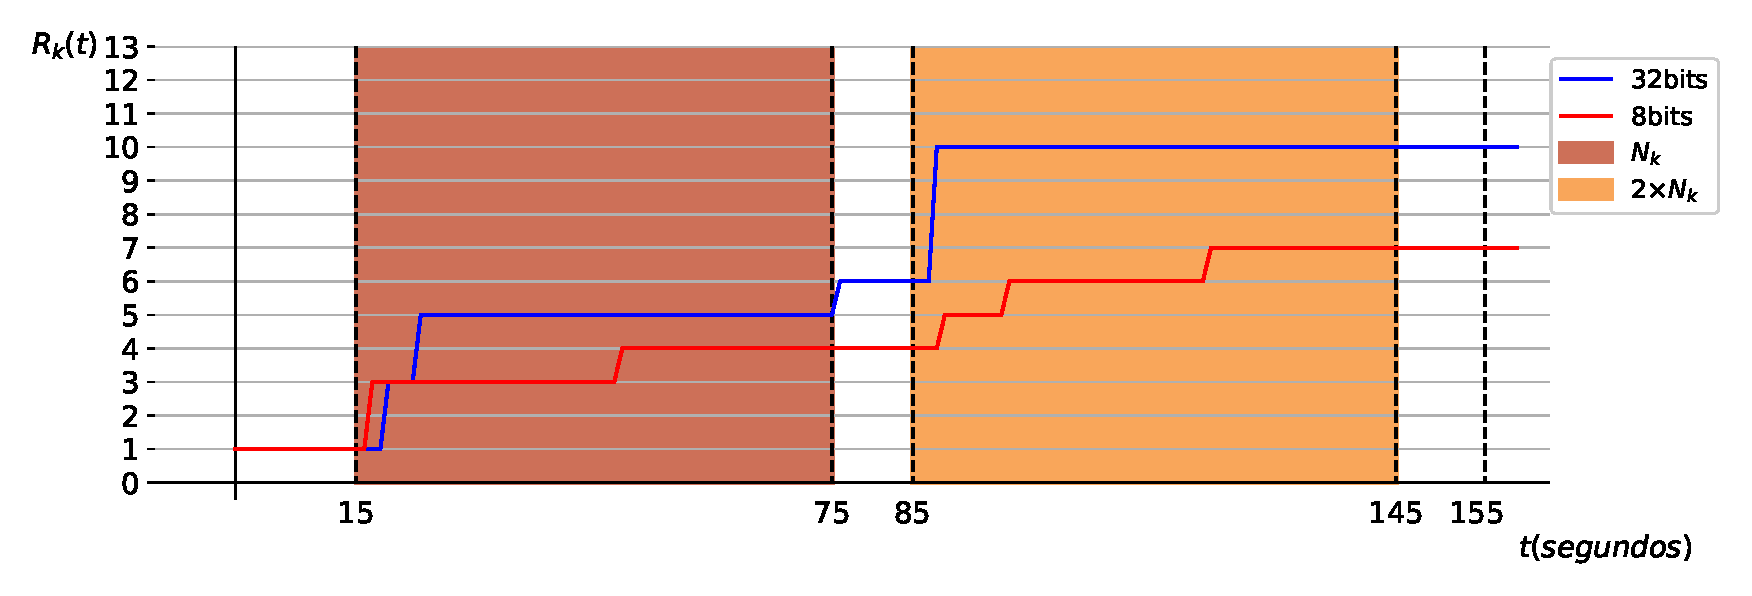
\includegraphics[width=1\textwidth]{figuras/escalonamento.eps}
    \caption{Comportamento da criação de novas réplicas com o passar do tempo do modelo não comprimido e quantizado em $8$ bits o primeiro perfil de estresse $N_1=75$.}
    \end{figure}
\end{frame}

\begin{frame}{Resultados}
    \begin{figure}[H]
    \centering
    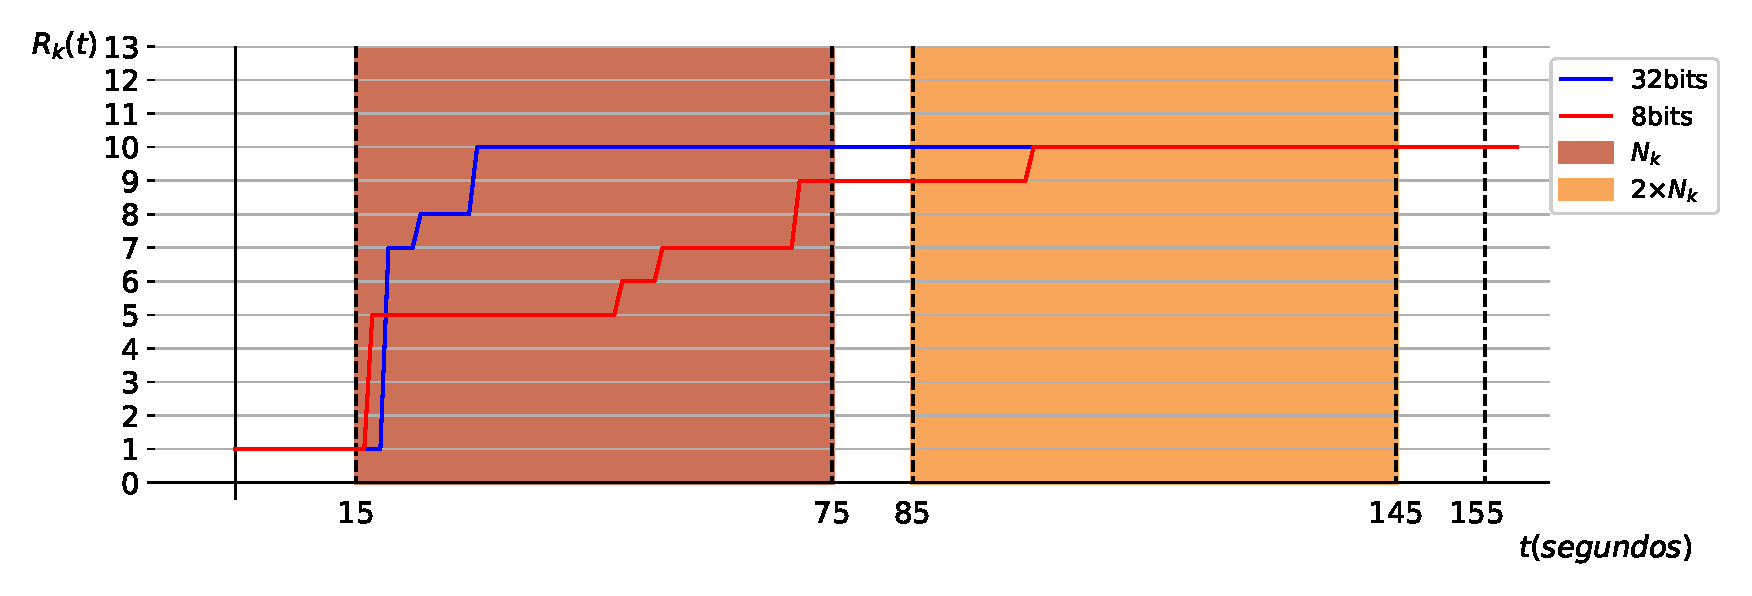
\includegraphics[width=1\textwidth]{figuras/escalonamento2.eps}
    \caption{Comportamento da criação de novas réplicas com o passar do tempo do modelo não comprimido e quantizado em $8$ bits o segundo perfil de estresse $N_2=125$.}
    \end{figure}
\end{frame}

\begin{frame}{Resultados}
    \begin{figure}[H]
    \centering
    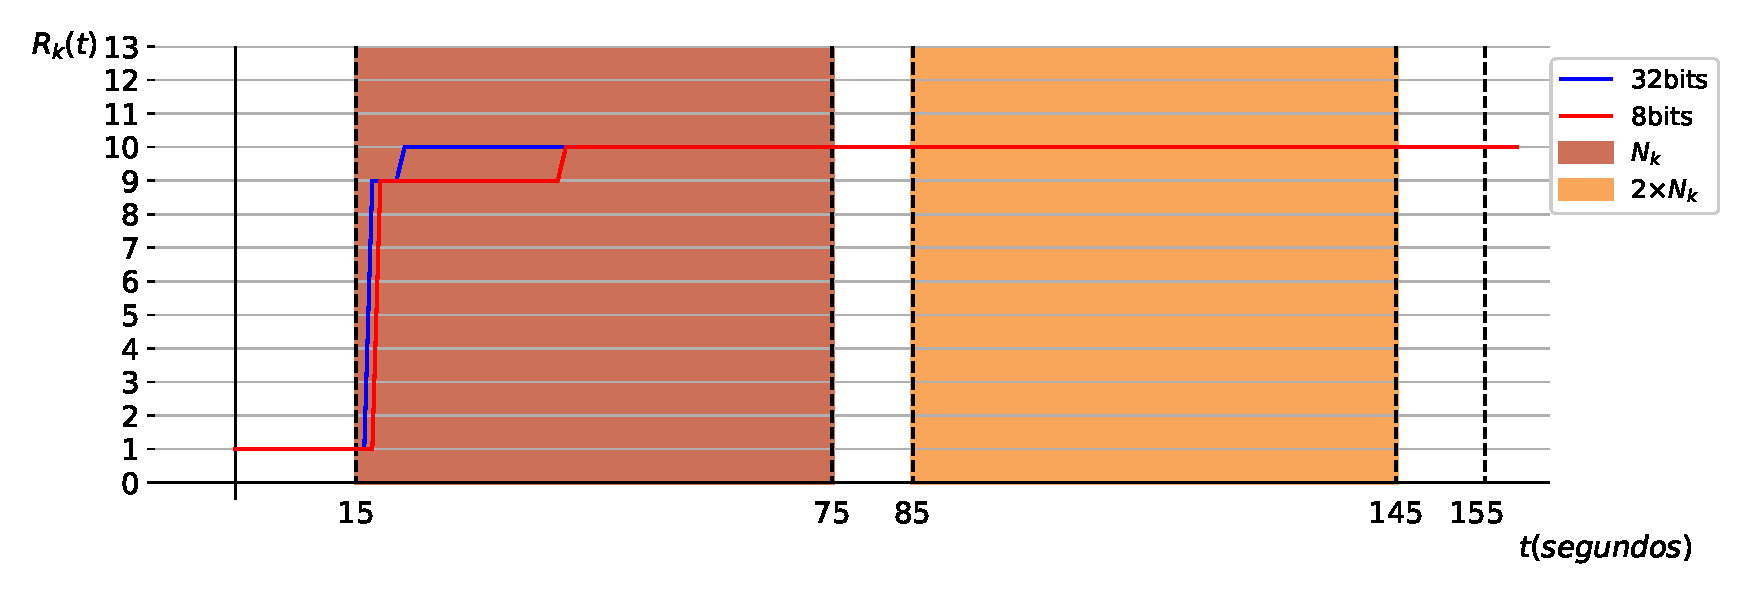
\includegraphics[width=1\textwidth]{figuras/escalonamento3.eps}
    \caption{Comportamento da criação de novas réplicas com o passar do tempo do modelo não comprimido e quantizado em $8$ bits o terceiro perfil de estresse $N_3=250$.}
    \end{figure}
\end{frame}